\chapter{Running Examples}

\section{Landing Page}
The landing page serves as the main entry point to the application. It provides users with a simple interface to begin their exploration. Users can search for places using the search bar.

\begin{figure}[H]
    \centering
    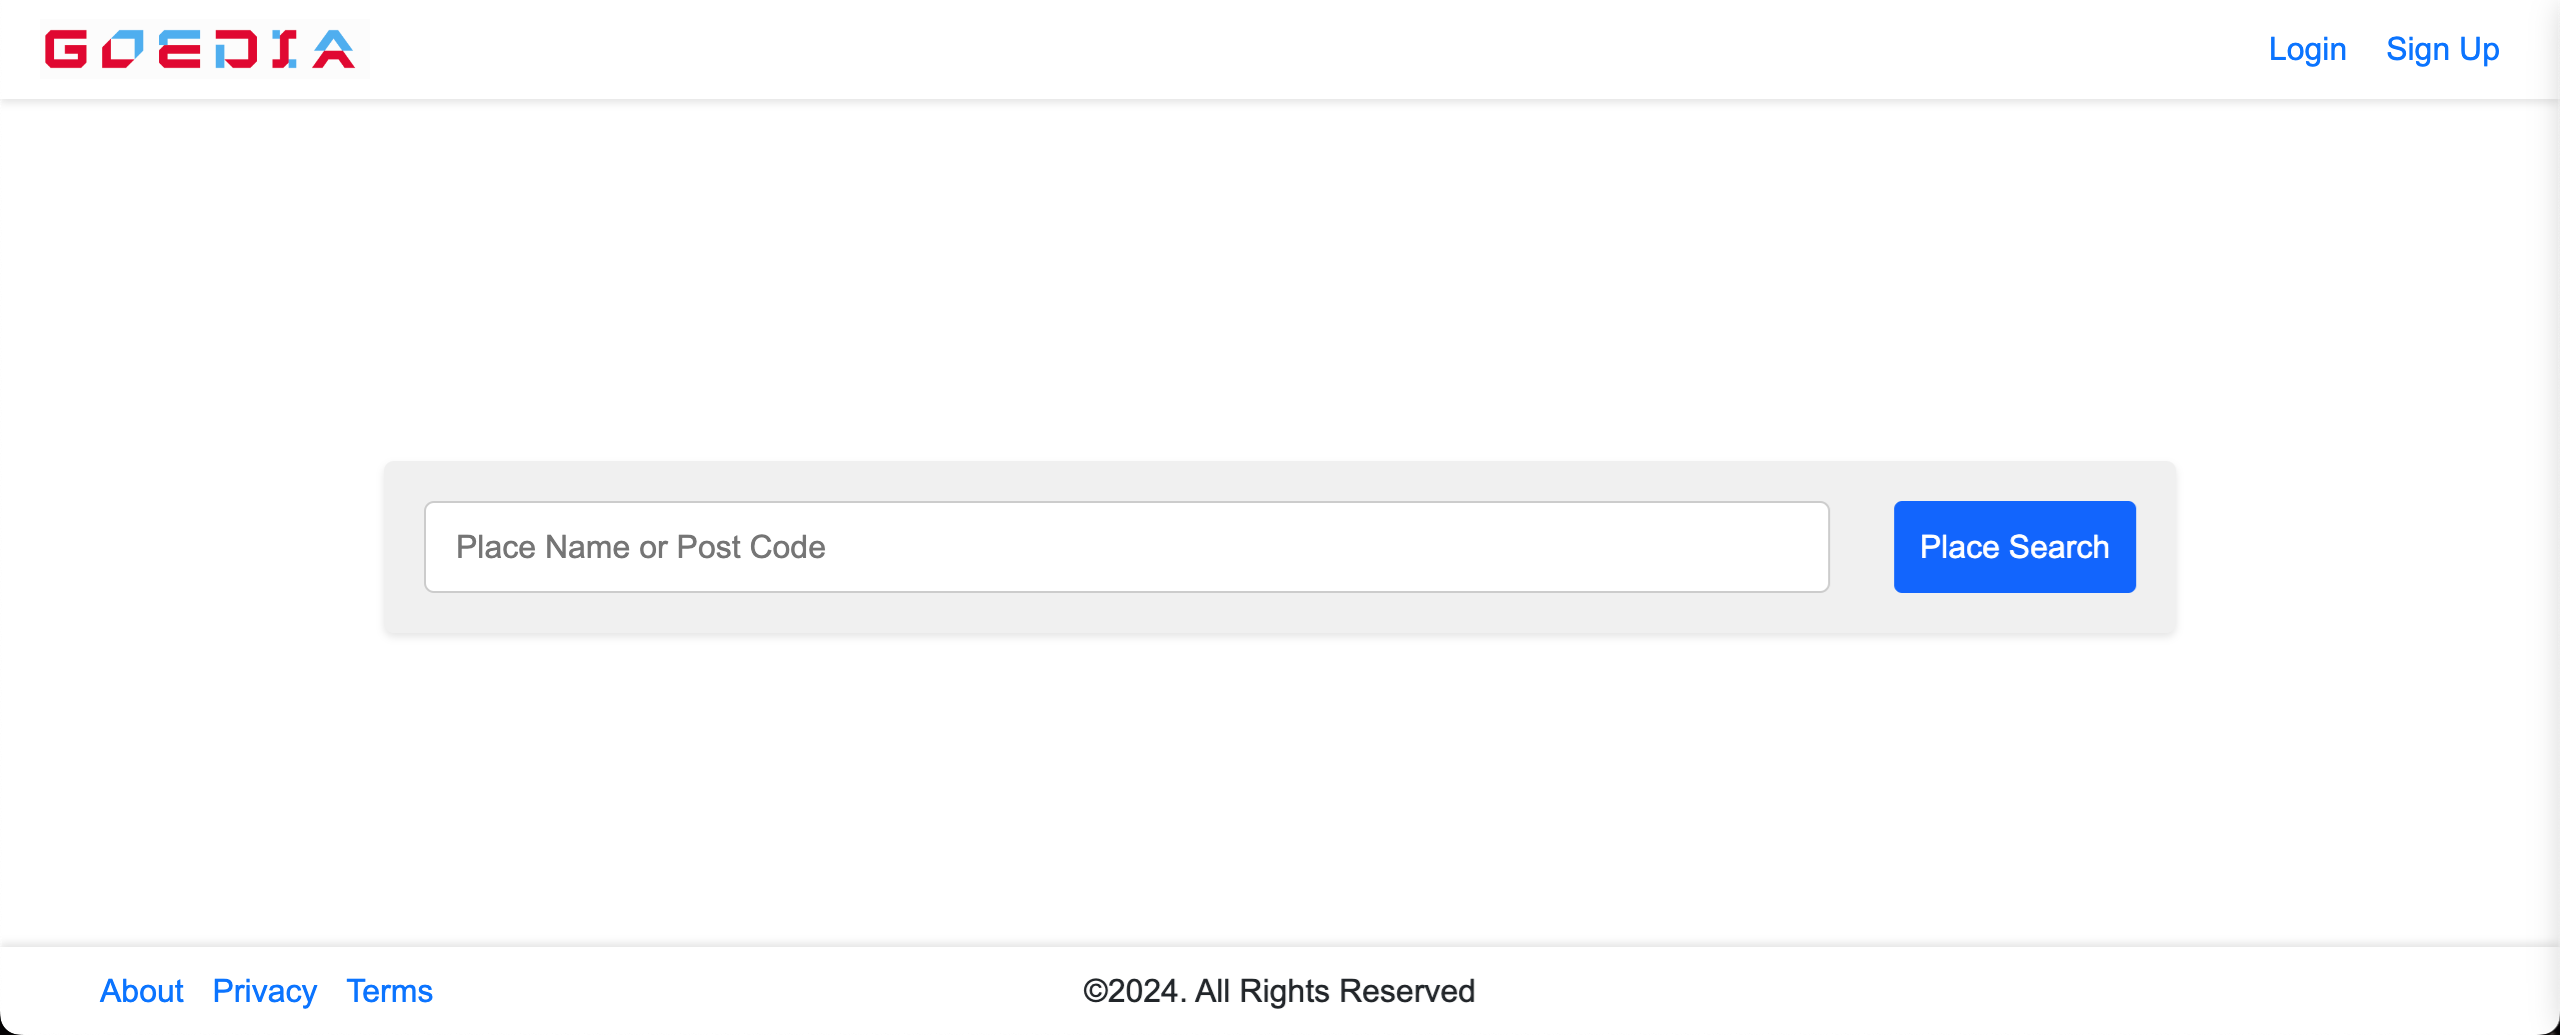
\includegraphics[width=\textwidth]{landingPage.png}
    \caption{Landing Page}
    \label{fig:landingPage}
\end{figure}

\section{Guest Search}
Guests can search for places without needing to log in. The search bar allows them to type in the name of a place, and suggestions are provided as they type.

\begin{figure}[H]
    \centering
    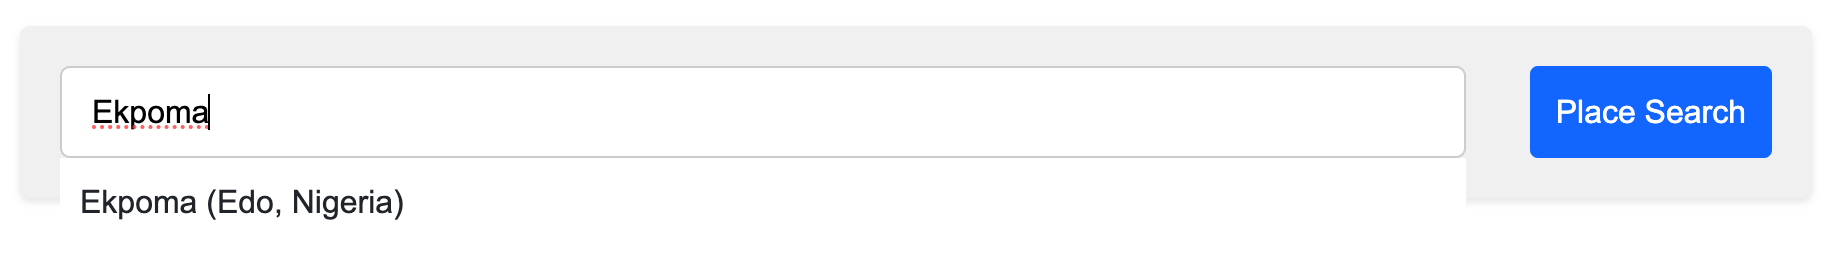
\includegraphics[width=\textwidth]{guestSearch.png}
    \caption{Guest Search}
    \label{fig:guestSearch}
\end{figure}

\section{Place Details}
When a place is selected, detailed information about it is displayed, including a map, the year it was founded, population, elevation, and a description. This helps users learn more about the place.

\begin{figure}[H]
    \centering
    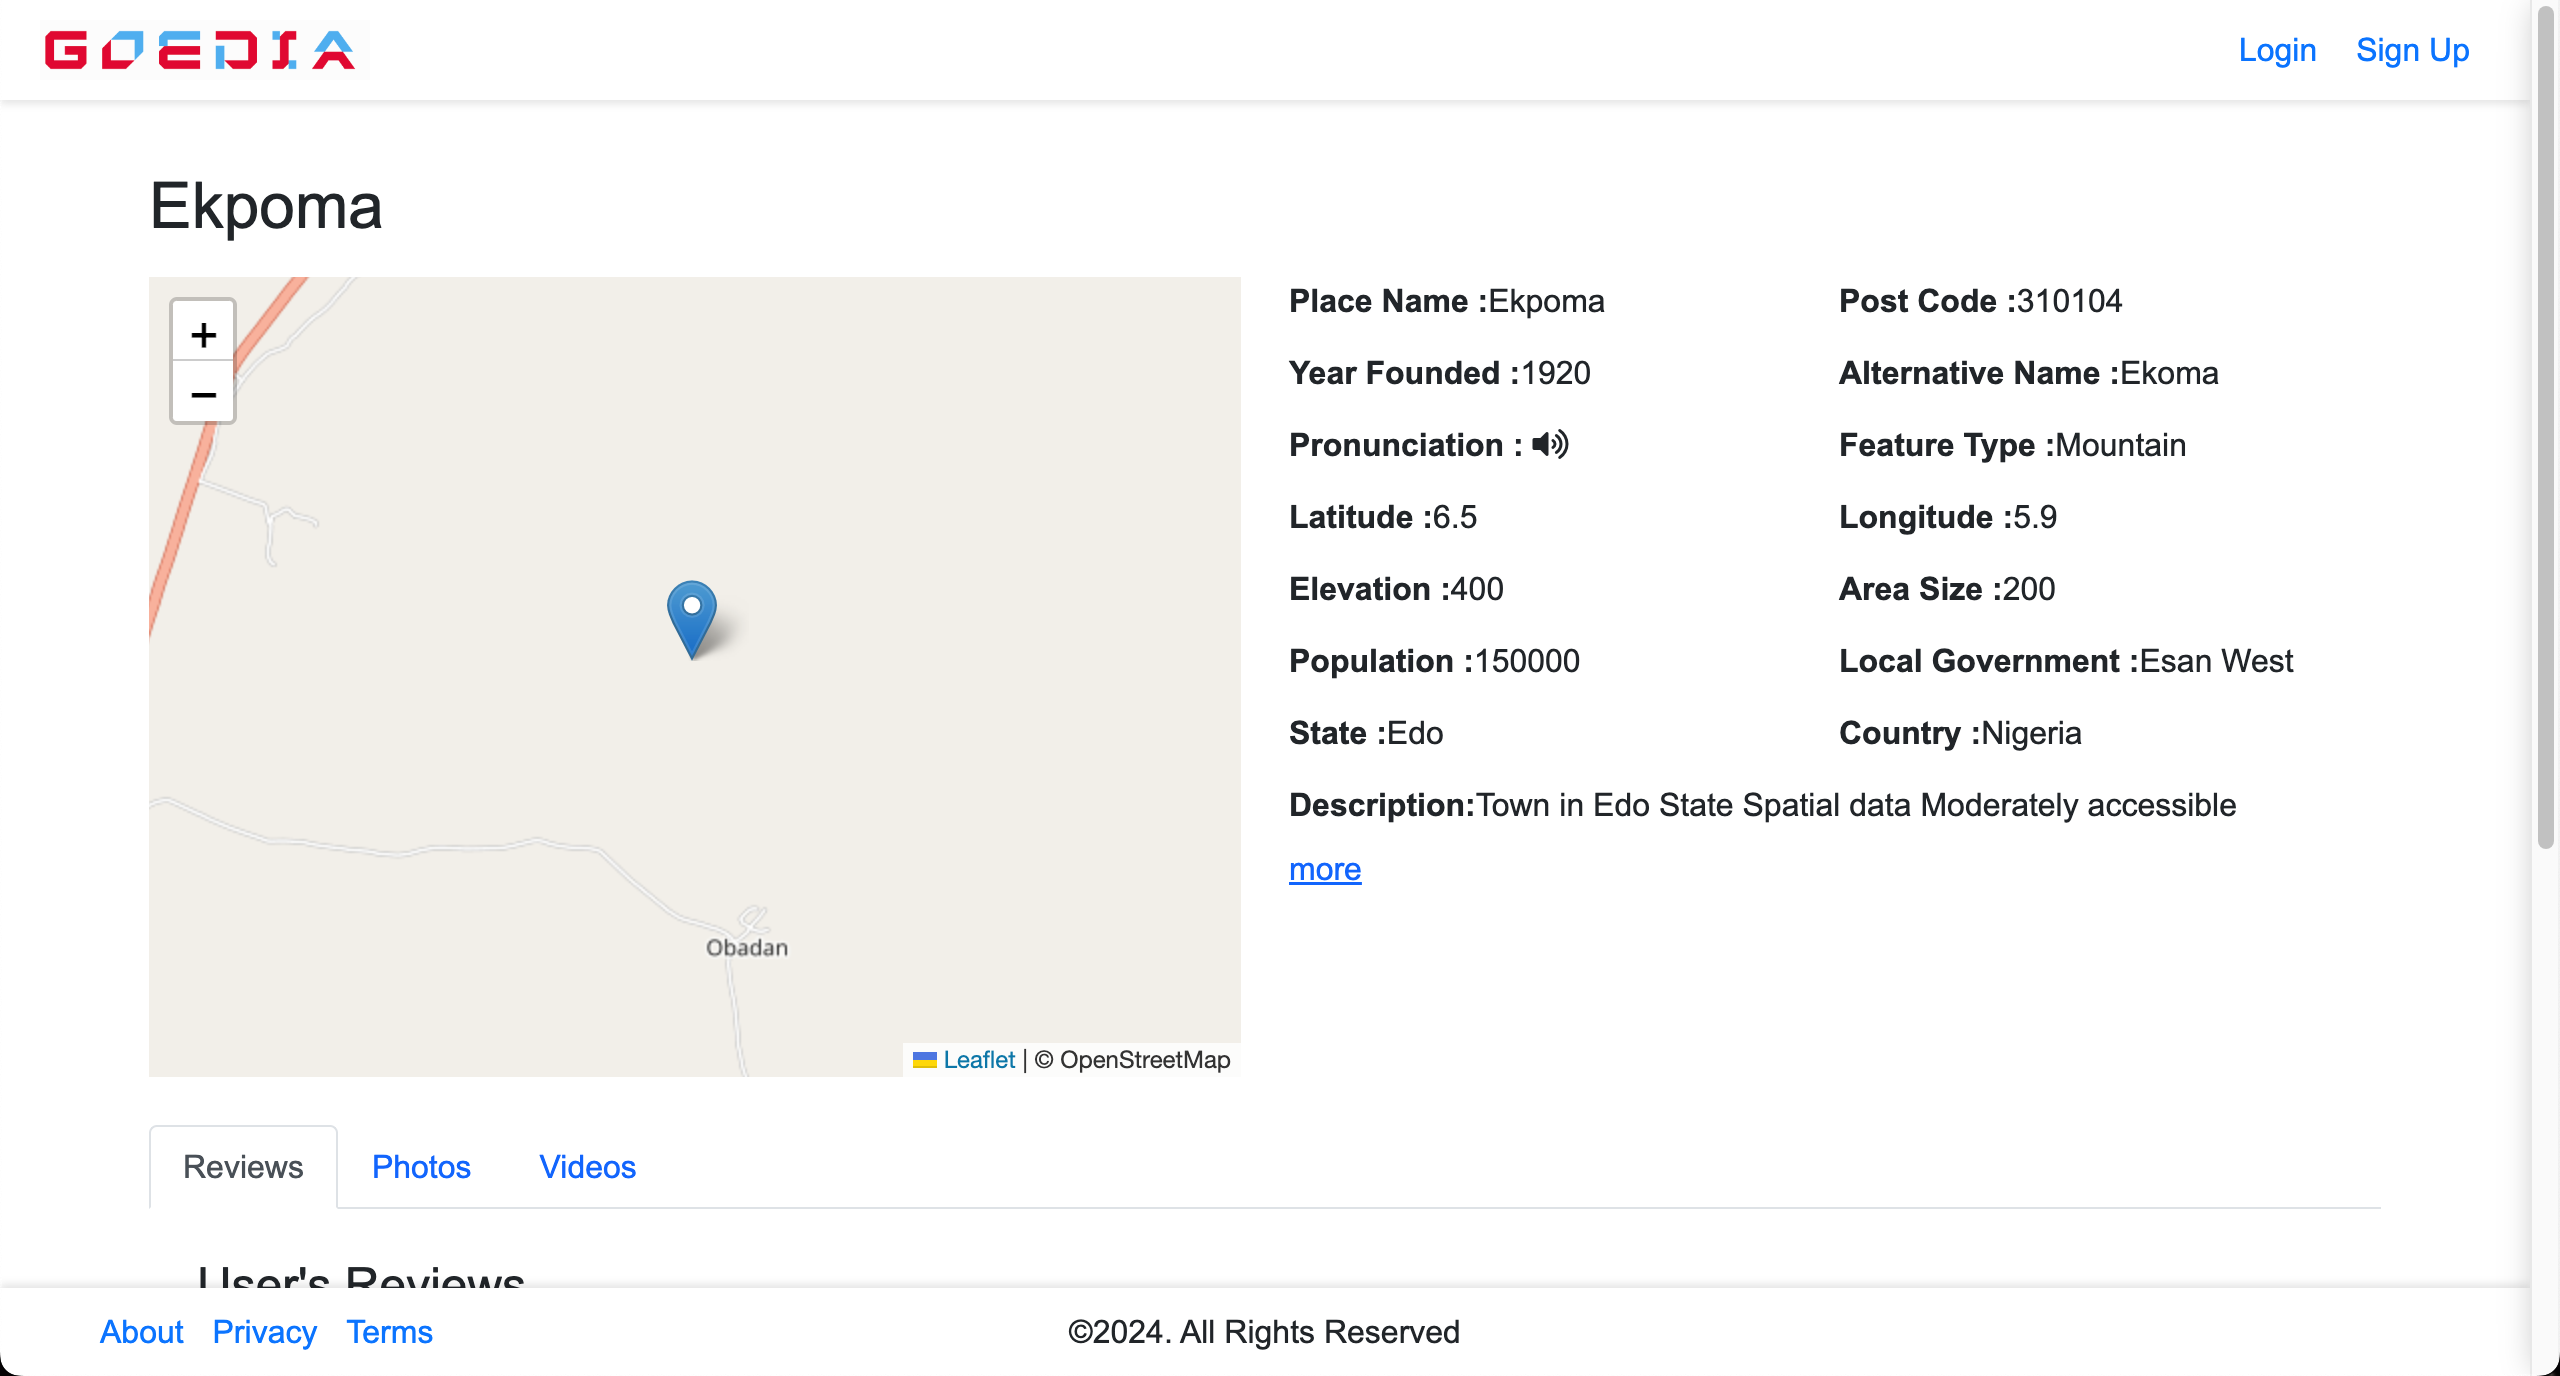
\includegraphics[width=\textwidth]{placeDetails.png}
    \caption{Place Details}
    \label{fig:placeDetails}
\end{figure}

\section{More Details}
Users can delve into additional details about a place. This section might include historical data, notable events, and other relevant information.

\begin{figure}[H]
    \centering
    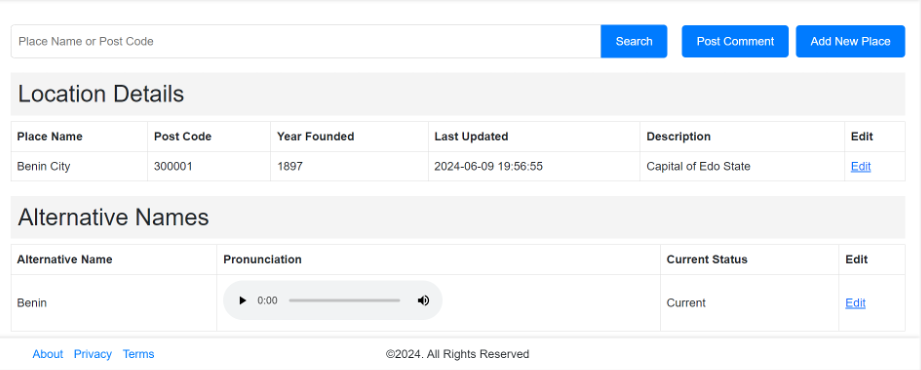
\includegraphics[width=\textwidth]{moreDetails.png}
    \caption{More Details}
    \label{fig:moreDetails}
\end{figure}

\section{Geographical Features}
This section provides geographical data about the place, such as its feature type, latitude, longitude, elevation, area size, and population. This information is useful for understanding the physical characteristics of the place.

\begin{figure}[H]
    \centering
    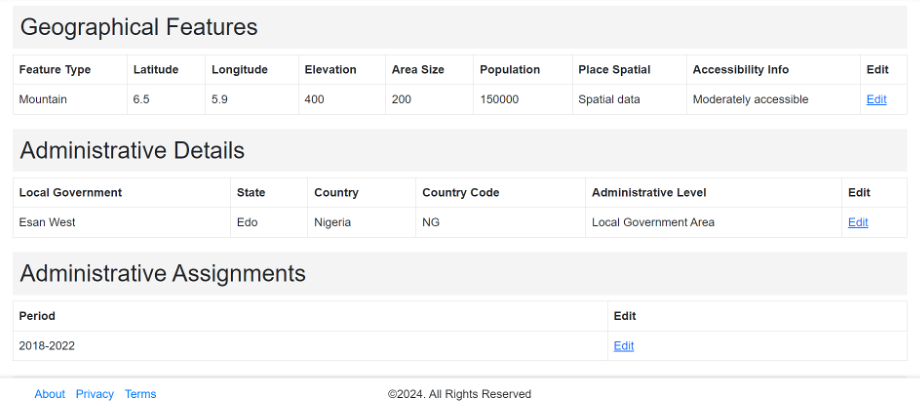
\includegraphics[width=\textwidth]{moreDetails2Geo.png}
    \caption{Geographical Features}
    \label{fig:moreDetails2Geo}
\end{figure}

\section{Administrative Details}
Additional administrative details about the place, such as the local government, state, country code, and administrative level, are provided here. This helps in identifying the place's governance and jurisdiction.

\begin{figure}[H]
    \centering
    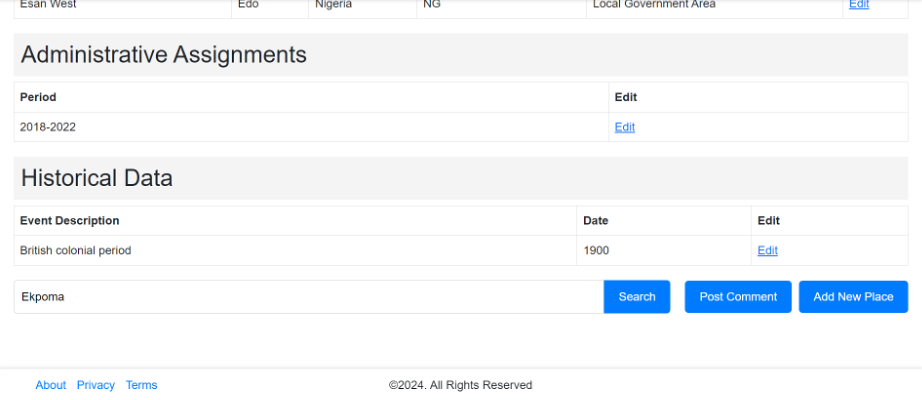
\includegraphics[width=\textwidth]{moreDetails3AdmDetails.png}
    \caption{Administrative Details}
    \label{fig:moreDetails3AdmDetails}
\end{figure}

\section{User Login}
Registered users can log in using their email address and password. This allows them to access personalized features and contribute content.

\begin{figure}[H]
    \centering
    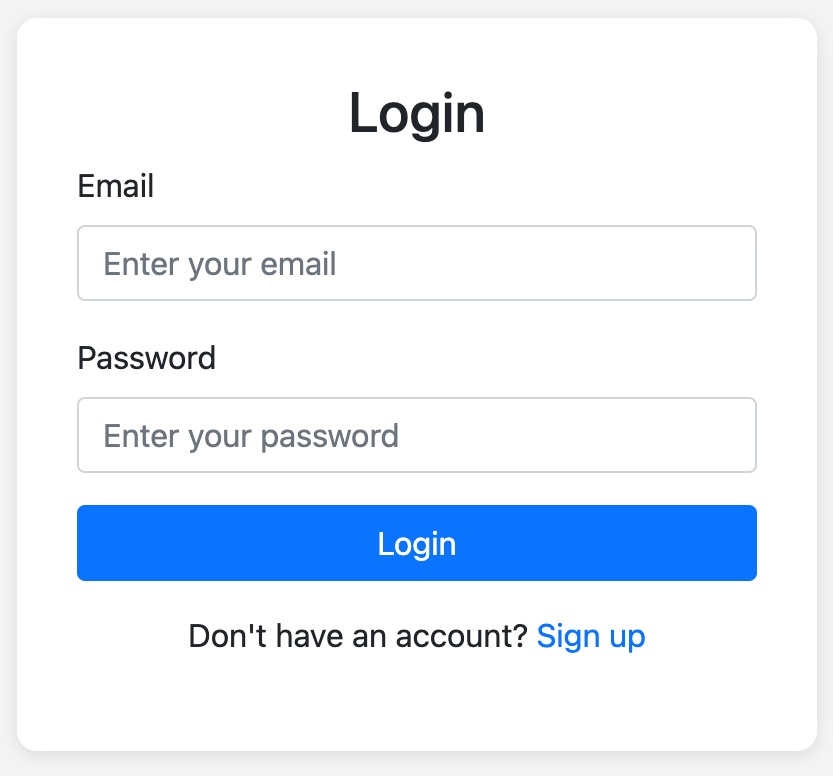
\includegraphics[width=\textwidth]{login.png}
    \caption{User Login}
    \label{fig:login}
\end{figure}

\section{User Registration}
New users can sign up by providing their full name, email address, password, and date of birth. This process allows them to create an account and start contributing to the platform.

\begin{figure}[H]
    \centering
    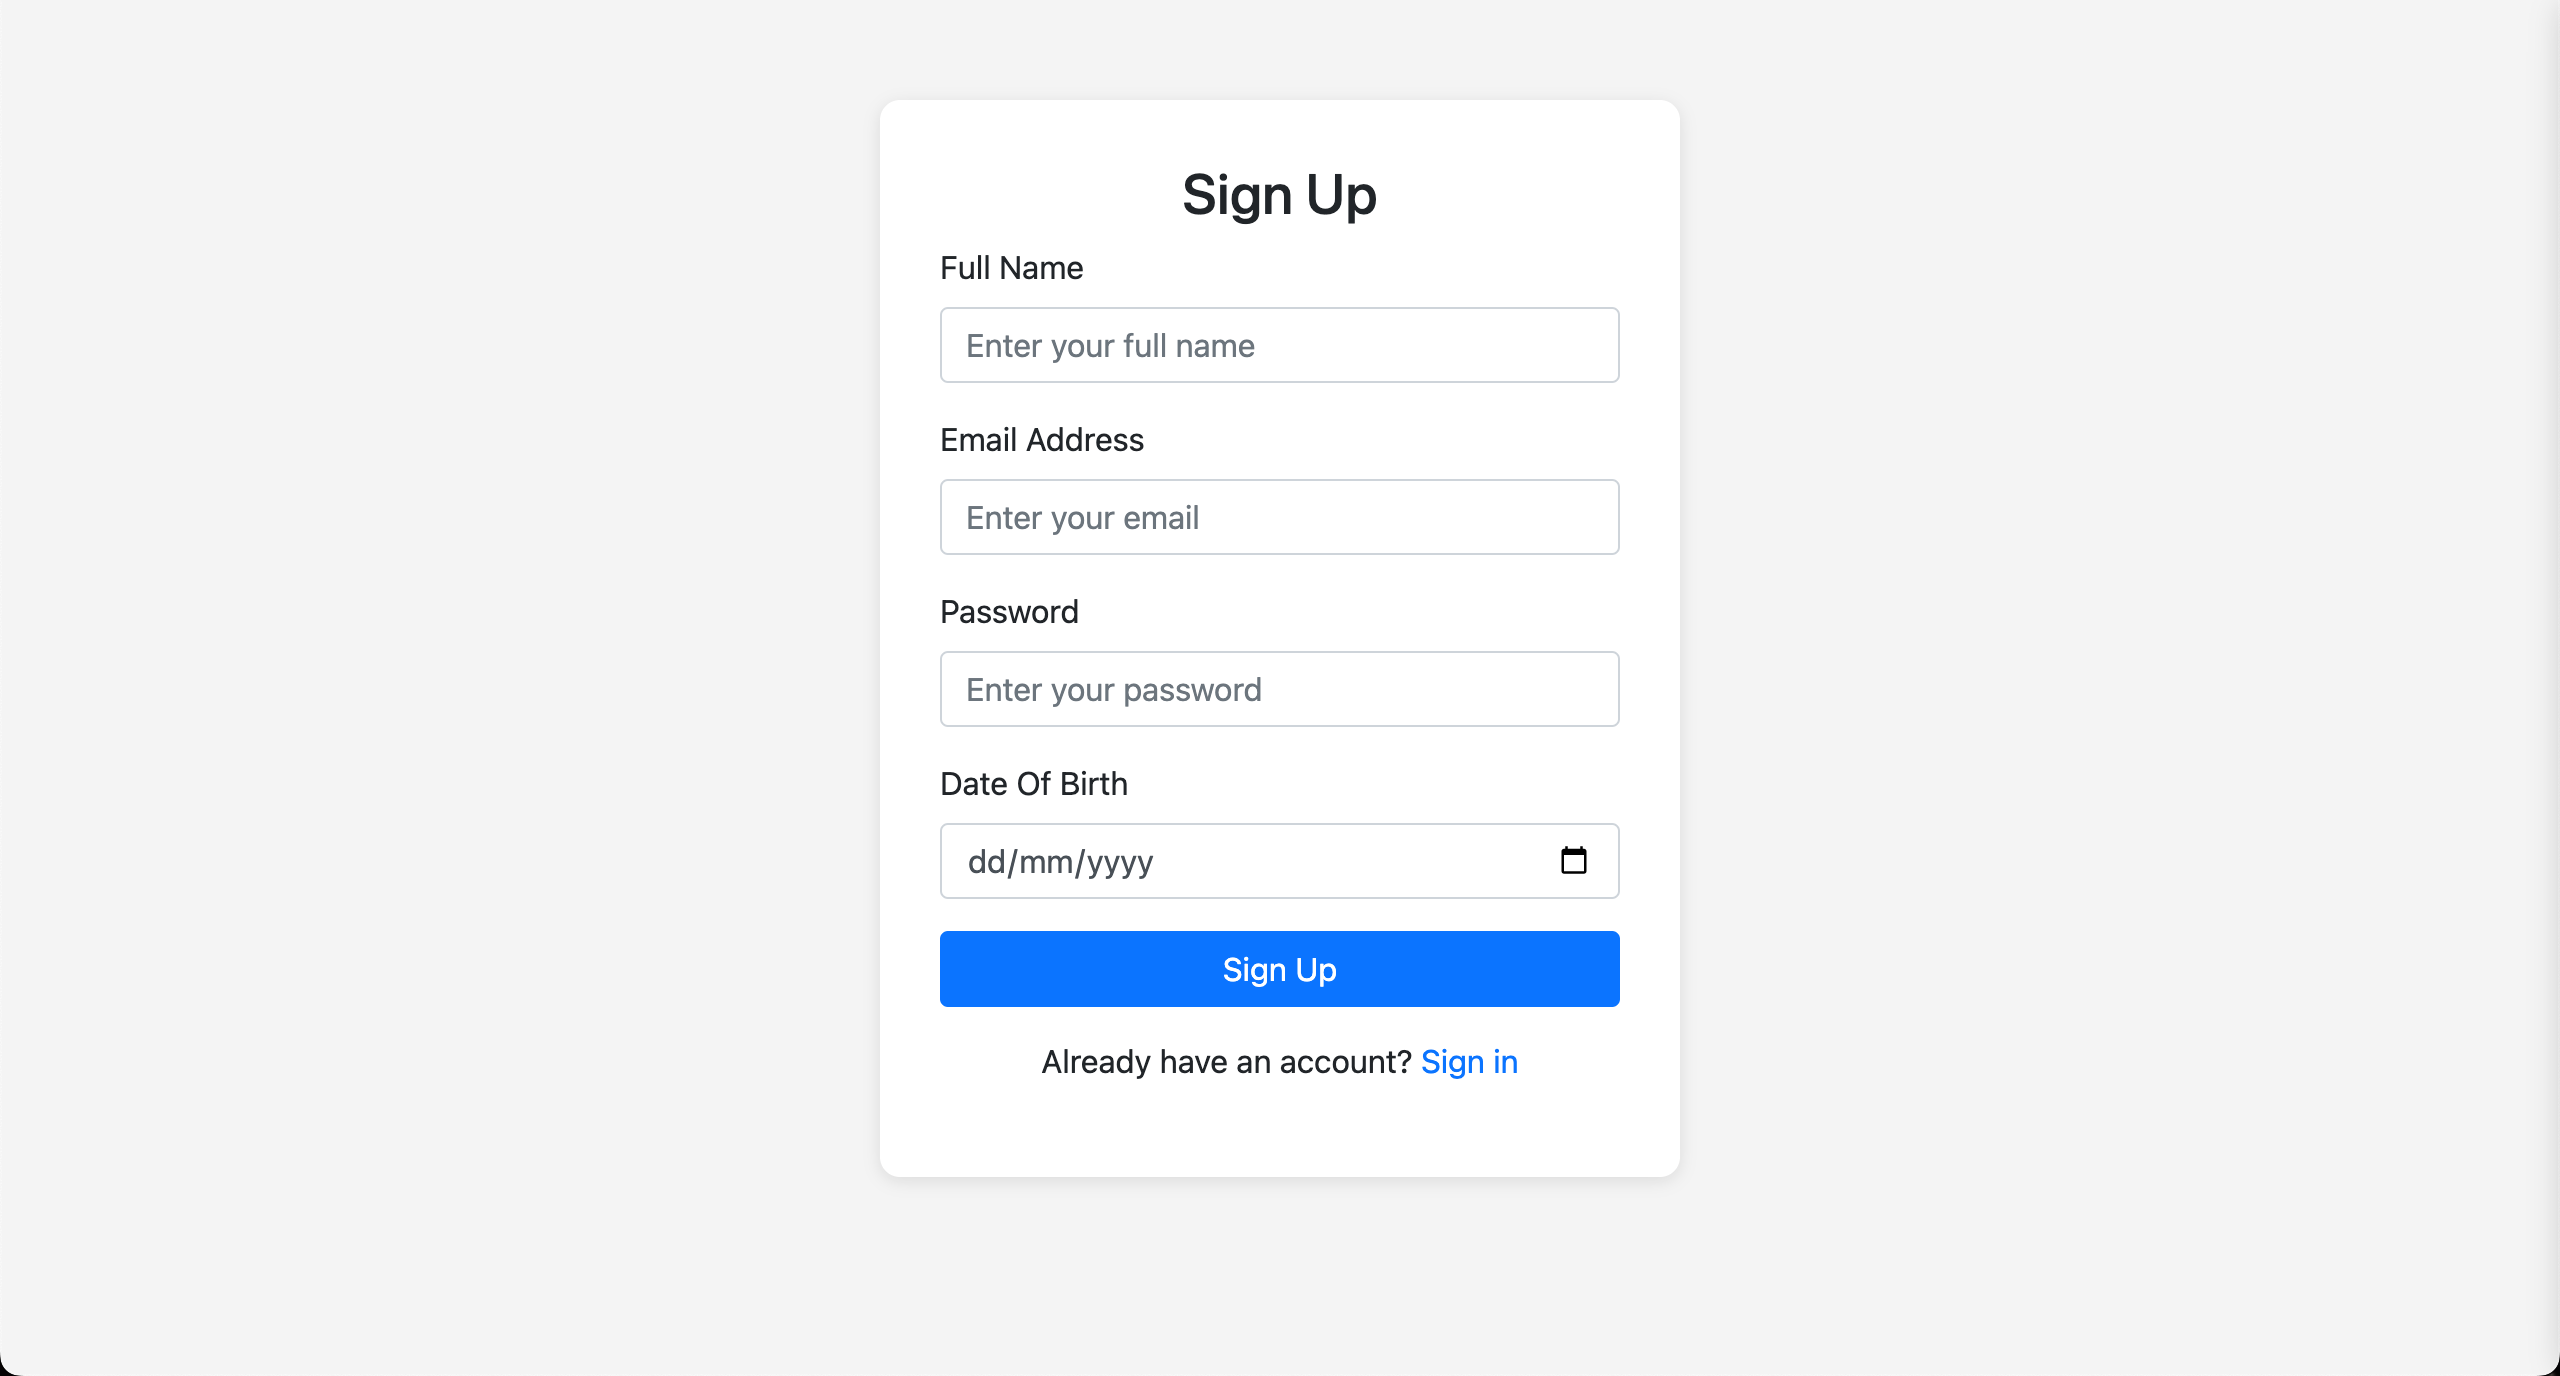
\includegraphics[width=\textwidth]{signup.png}
    \caption{User Registration}
    \label{fig:signup}
\end{figure}

\section{Add New Place - Basic Information}
Users can add new places by filling in basic information such as the place name, post code, year founded, and a brief description.

\begin{figure}[H]
    \centering
    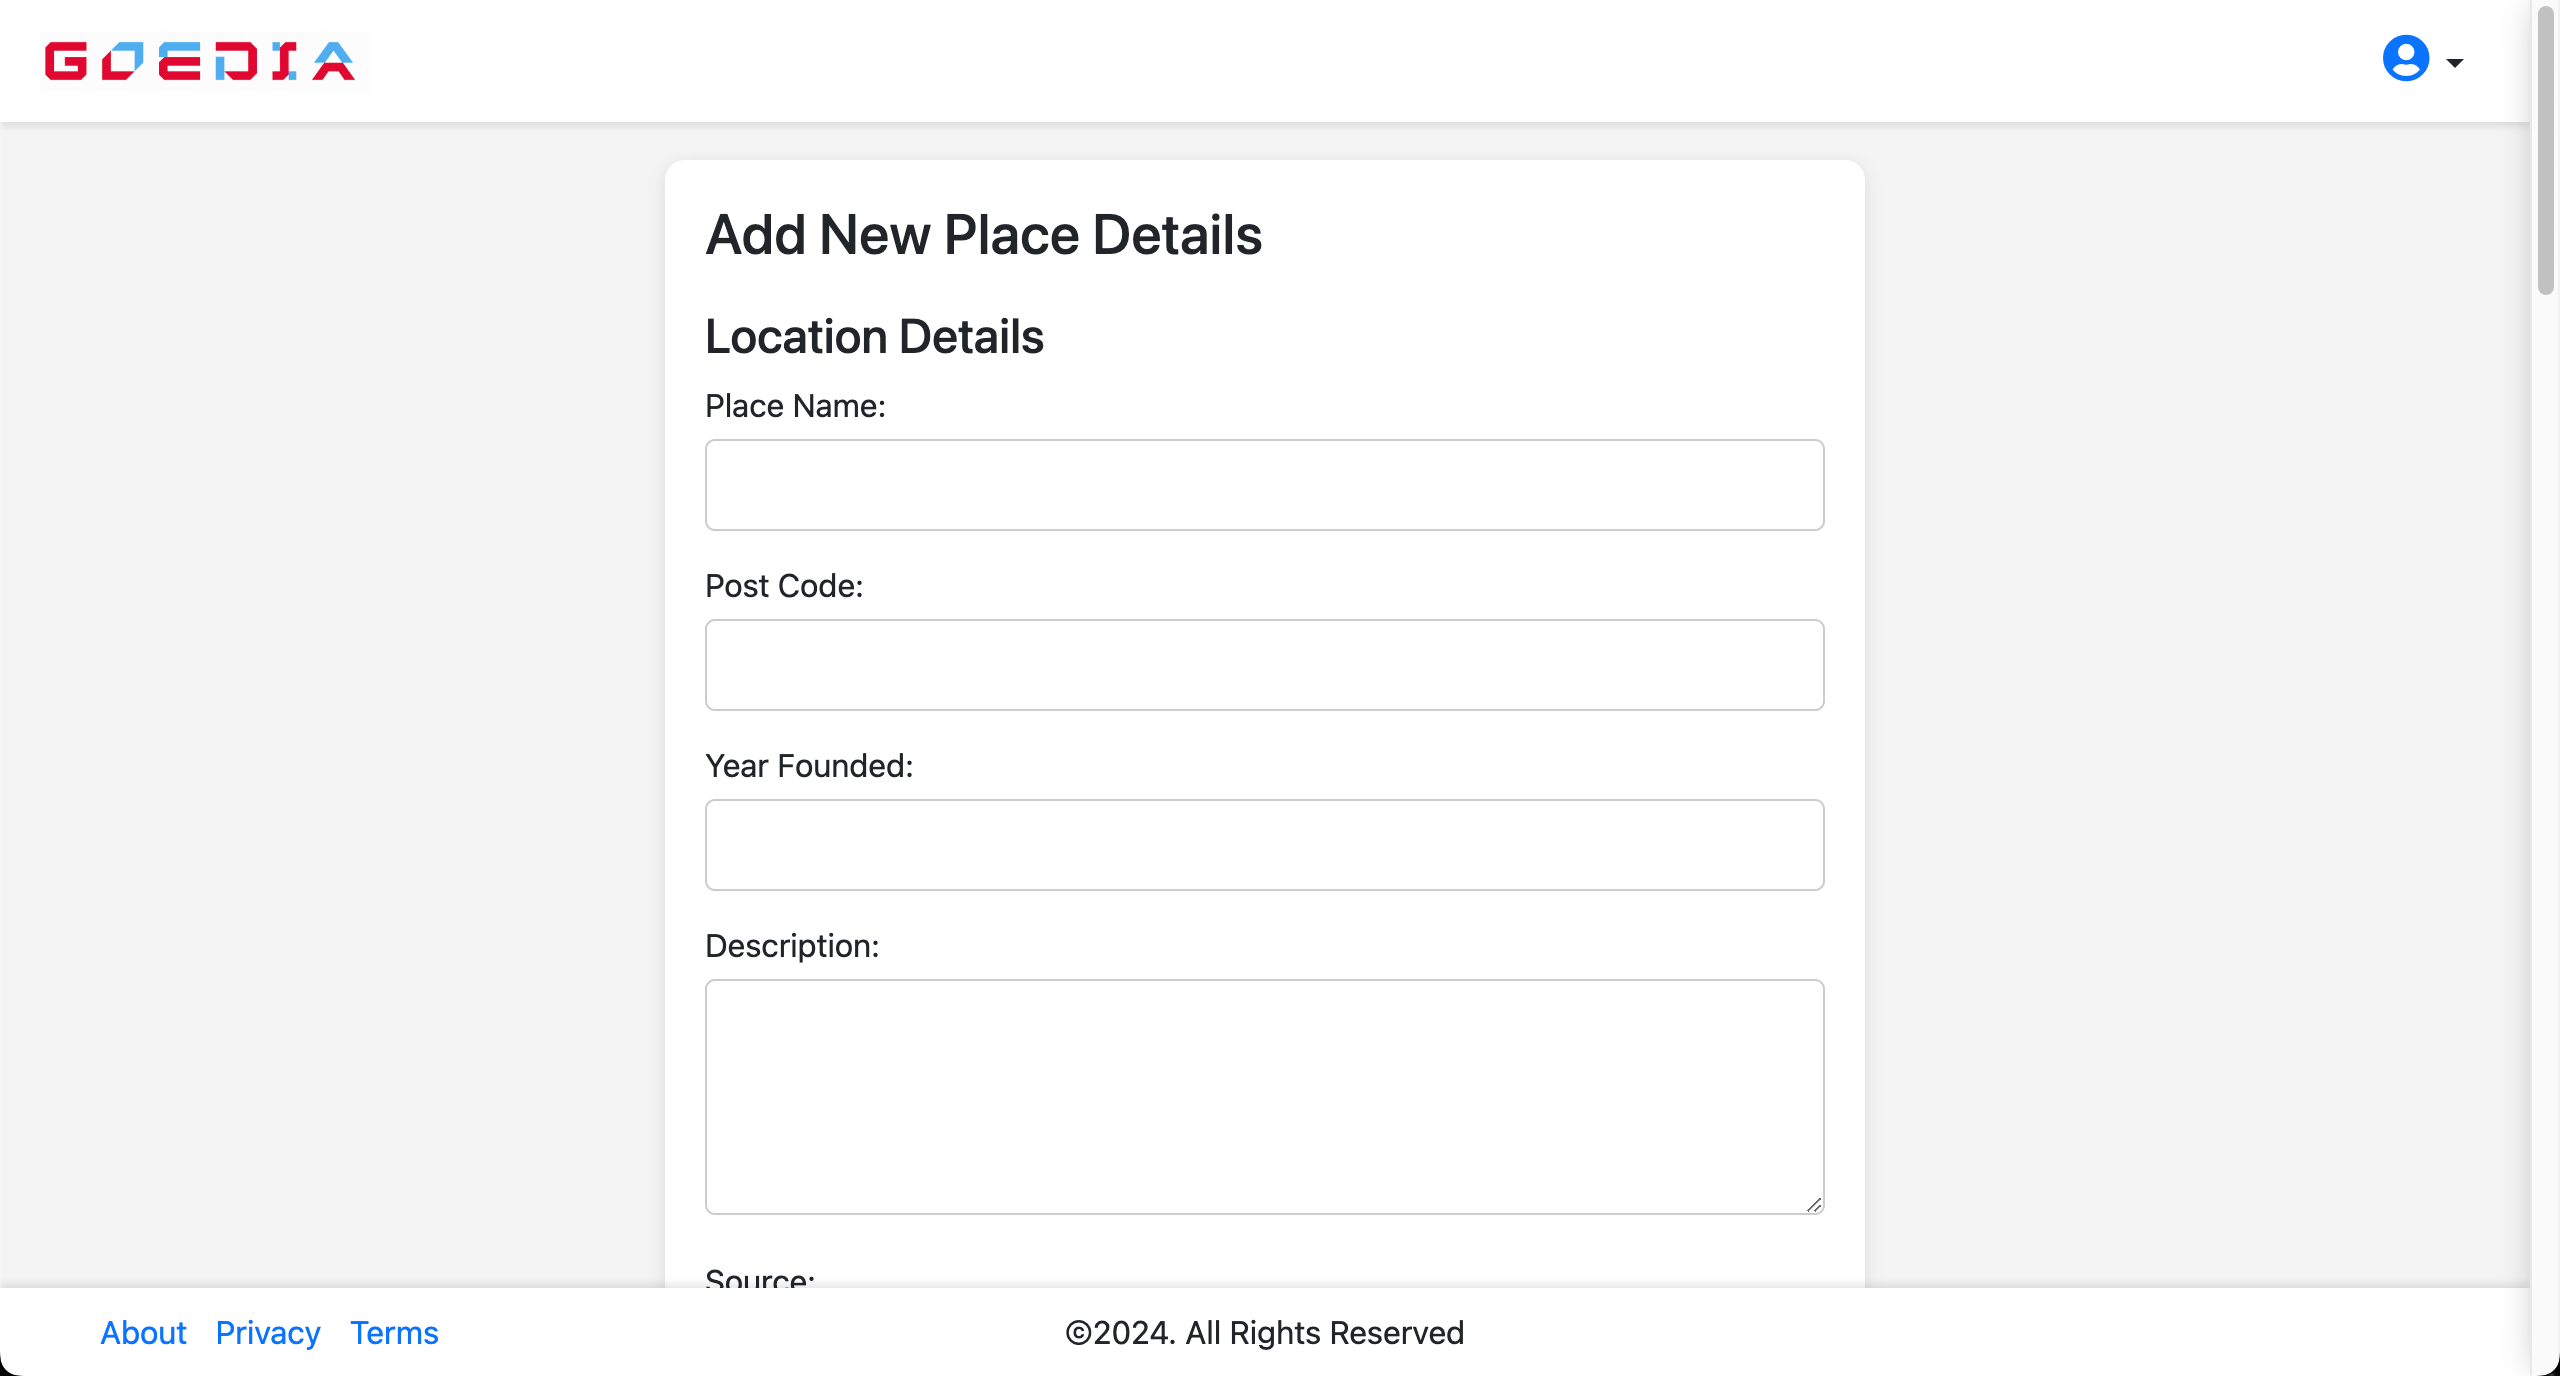
\includegraphics[width=\textwidth]{addnewPlace.png}
    \caption{Add New Place - Basic Information}
    \label{fig:addnewPlace}
\end{figure}

\section{Add New Place - Alternative Names}
Users can provide alternative names for a place, along with their pronunciation. This section also includes options to indicate if the name is currently in use and to add historical data.

\begin{figure}[H]
    \centering
    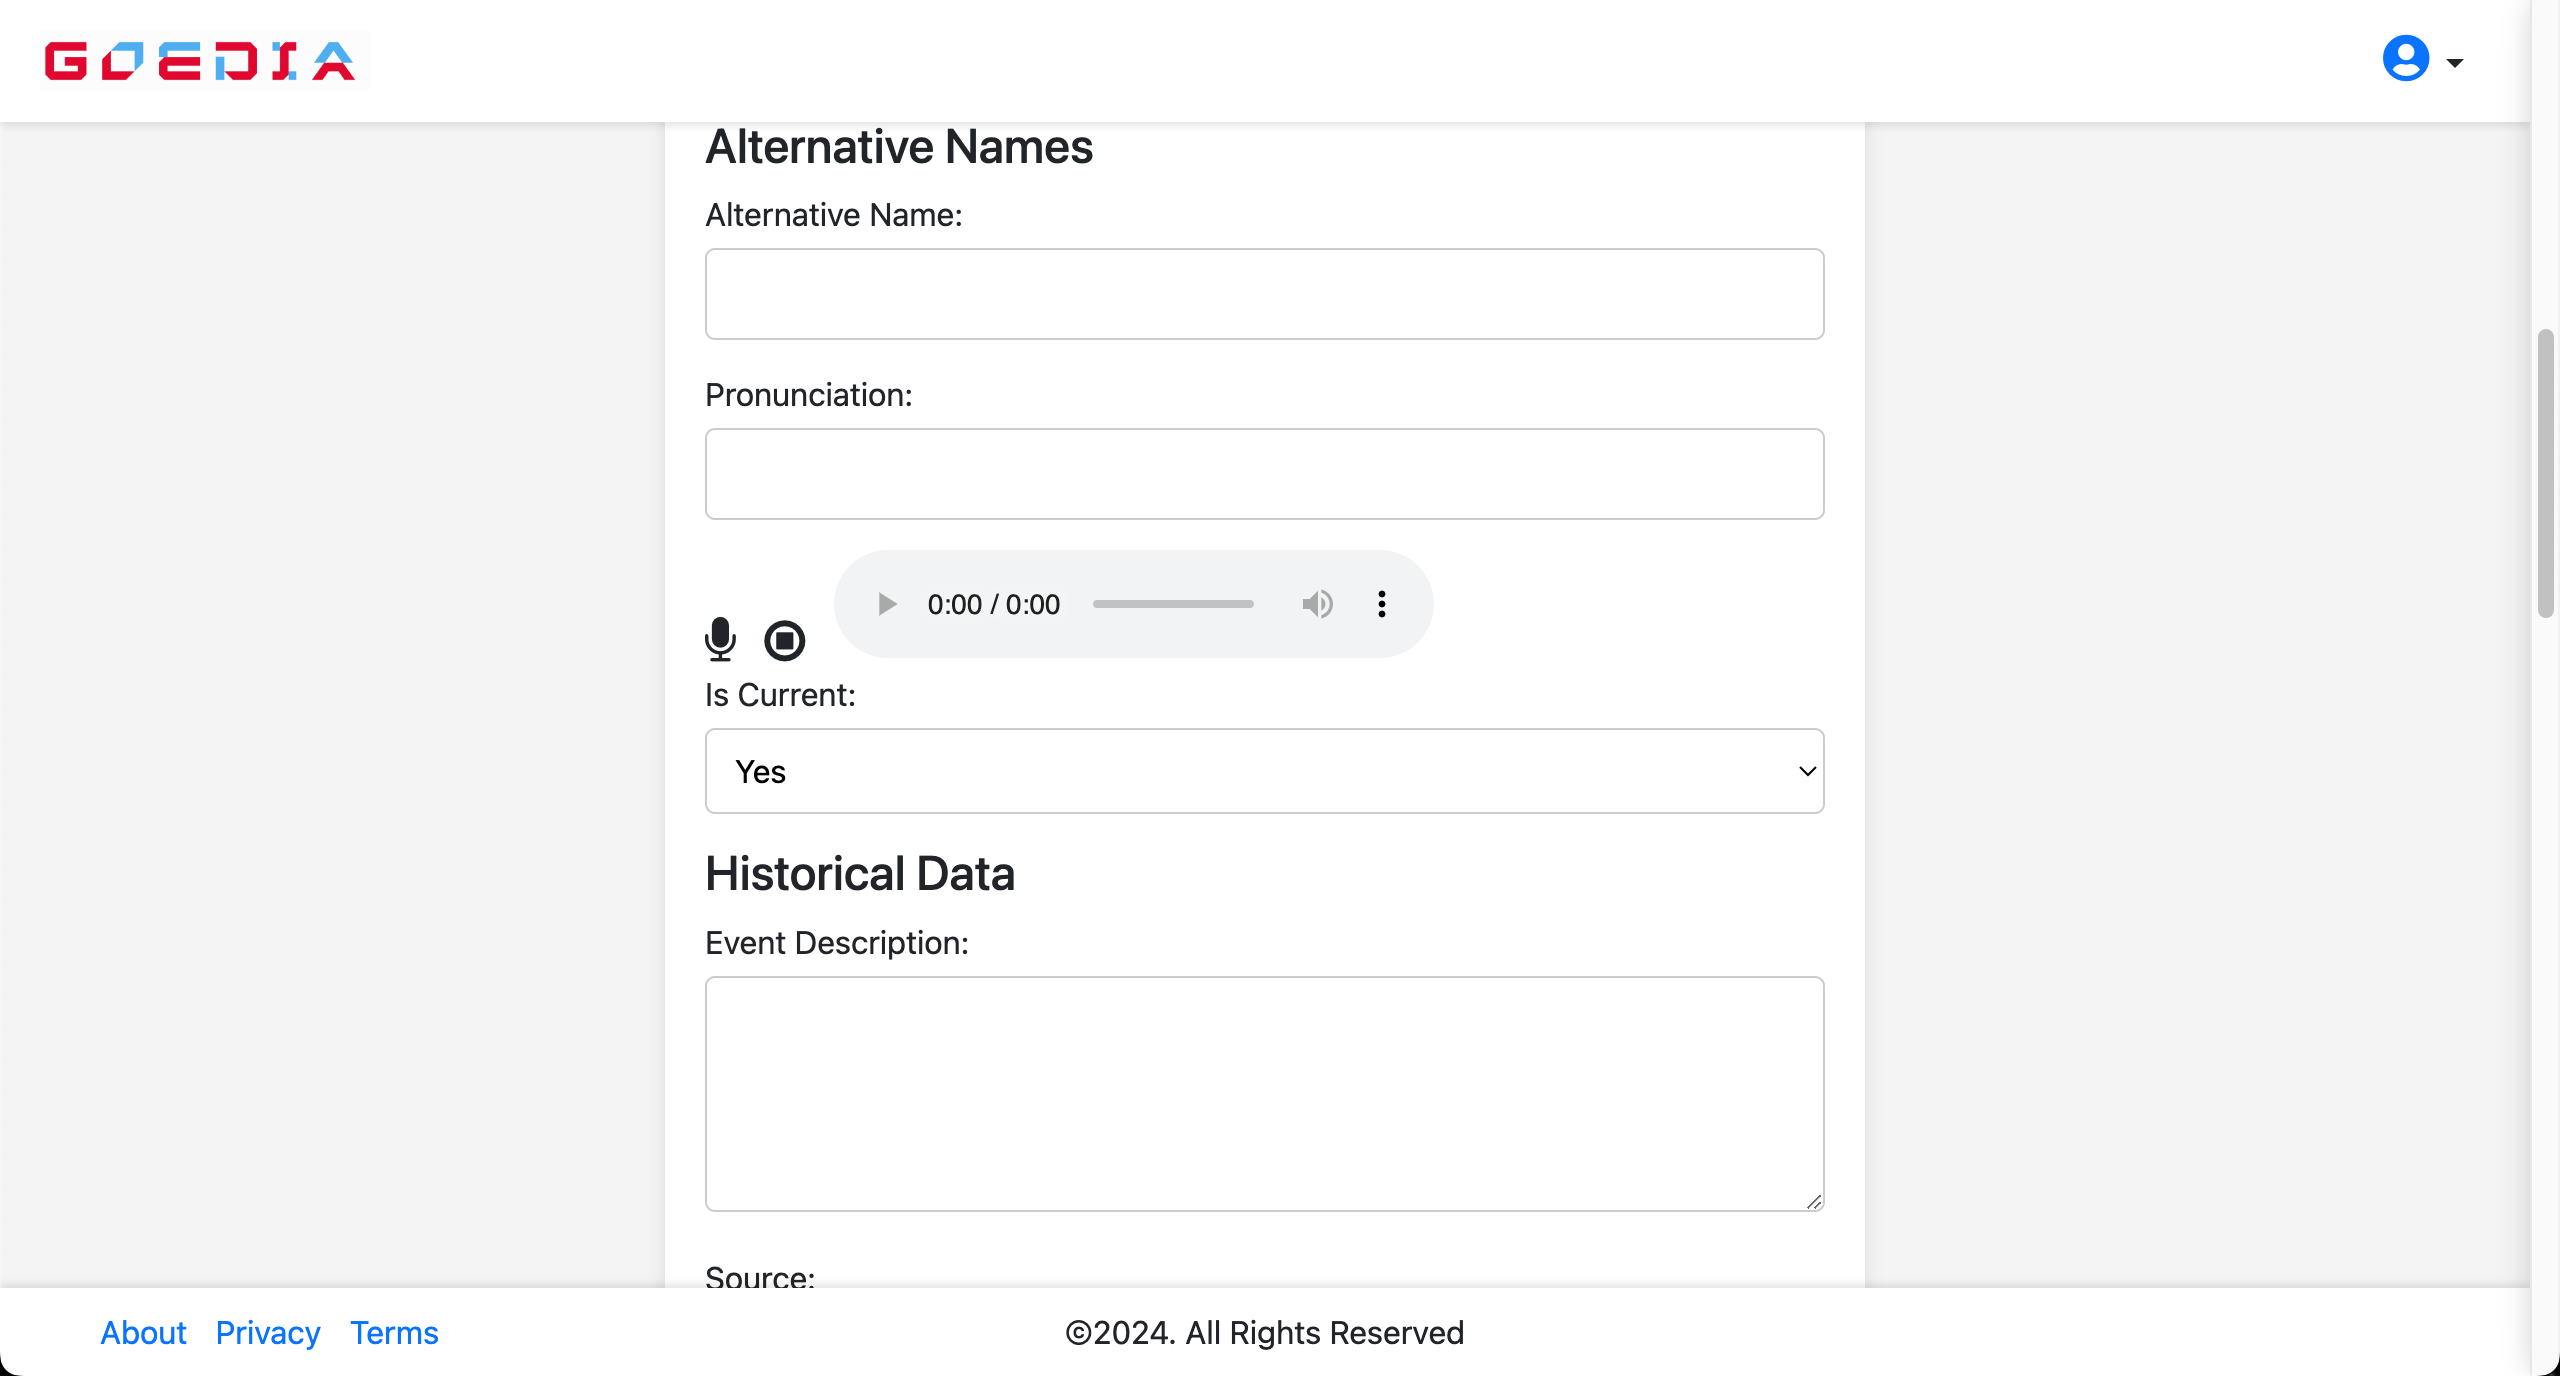
\includegraphics[width=\textwidth]{addnewPlaceAlternativeName.png}
    \caption{Add New Place - Alternative Names}
    \label{fig:addnewPlaceAlternativeName}
\end{figure}

\section{Add New Place - Geographical Features}
Geographical details such as the feature type, latitude, longitude, elevation, area size, and population are entered here to give a comprehensive understanding of the place's physical characteristics.

\begin{figure}[H]
    \centering
    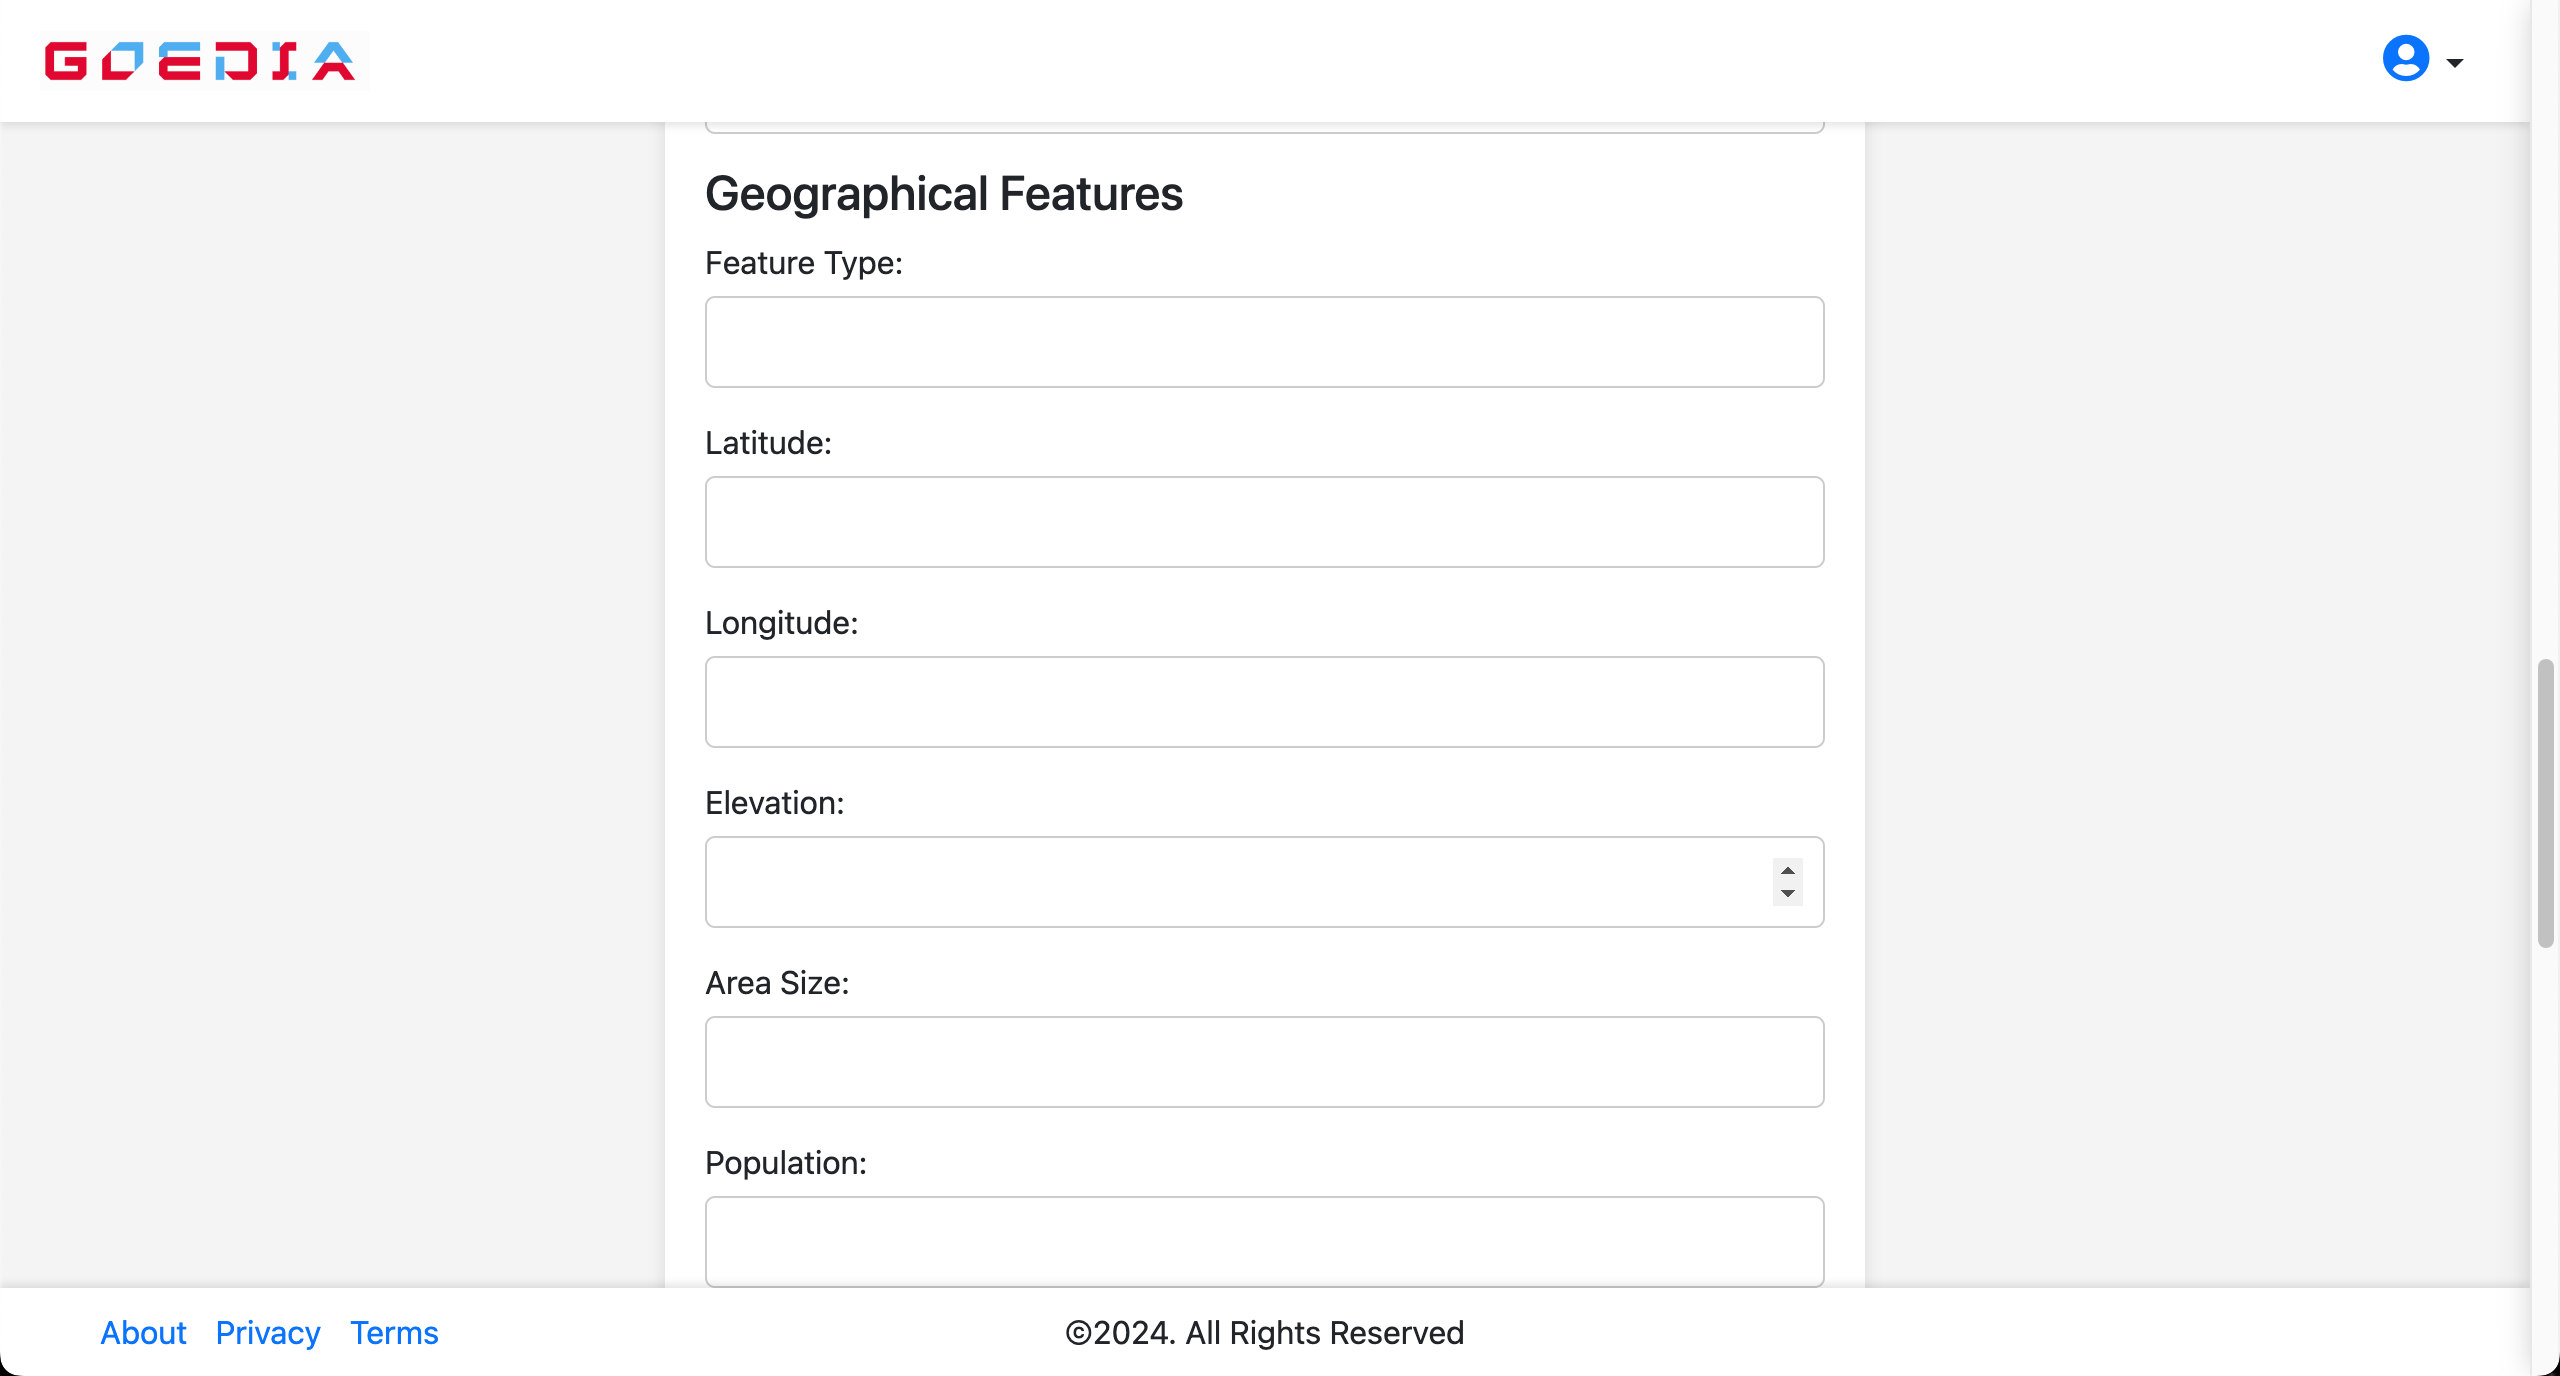
\includegraphics[width=\textwidth]{addnewPlaceGeo.png}
    \caption{Add New Place - Geographical Features}
    \label{fig:addnewPlaceGeo}
\end{figure}

\section{Add New Place - Administrative Details}
Users can add administrative details such as the local government, state, country code, country, and administrative level to provide more context about the governance of the place.

\begin{figure}[H]
    \centering
    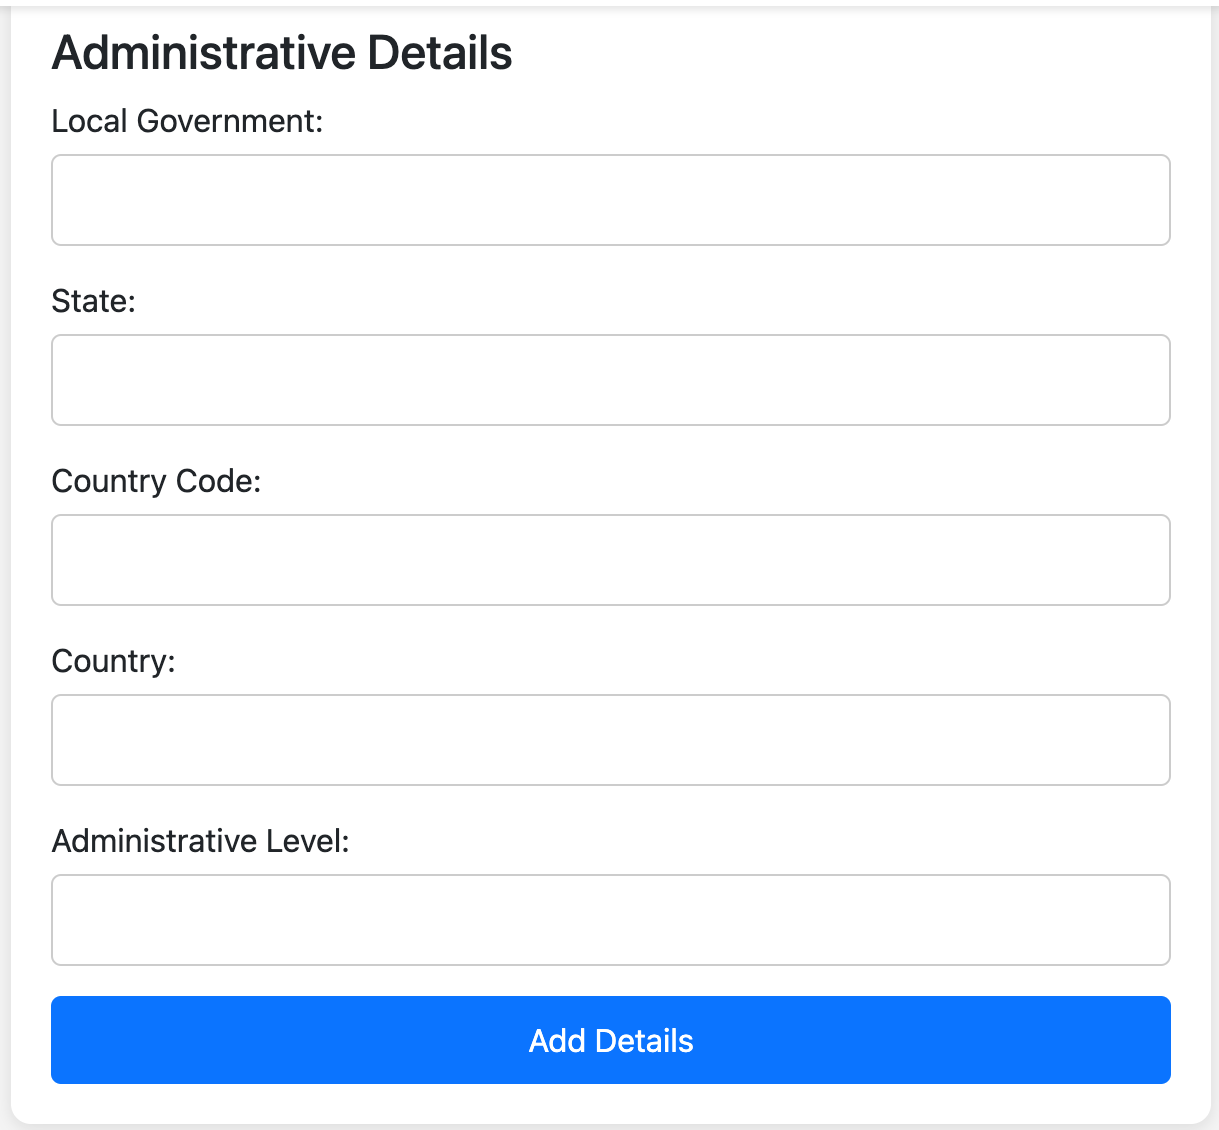
\includegraphics[width=\textwidth]{addNewPlaceAdmDetails.png}
    \caption{Add New Place - Administrative Details}
    \label{fig:addNewPlaceAdmDetails}
\end{figure}

\section{Experience Feed}
Users can view and share their experiences about different places. The feed displays user posts along with the date and time they were shared, providing a platform for users to share their stories and insights.

\begin{figure}[H]
    \centering
    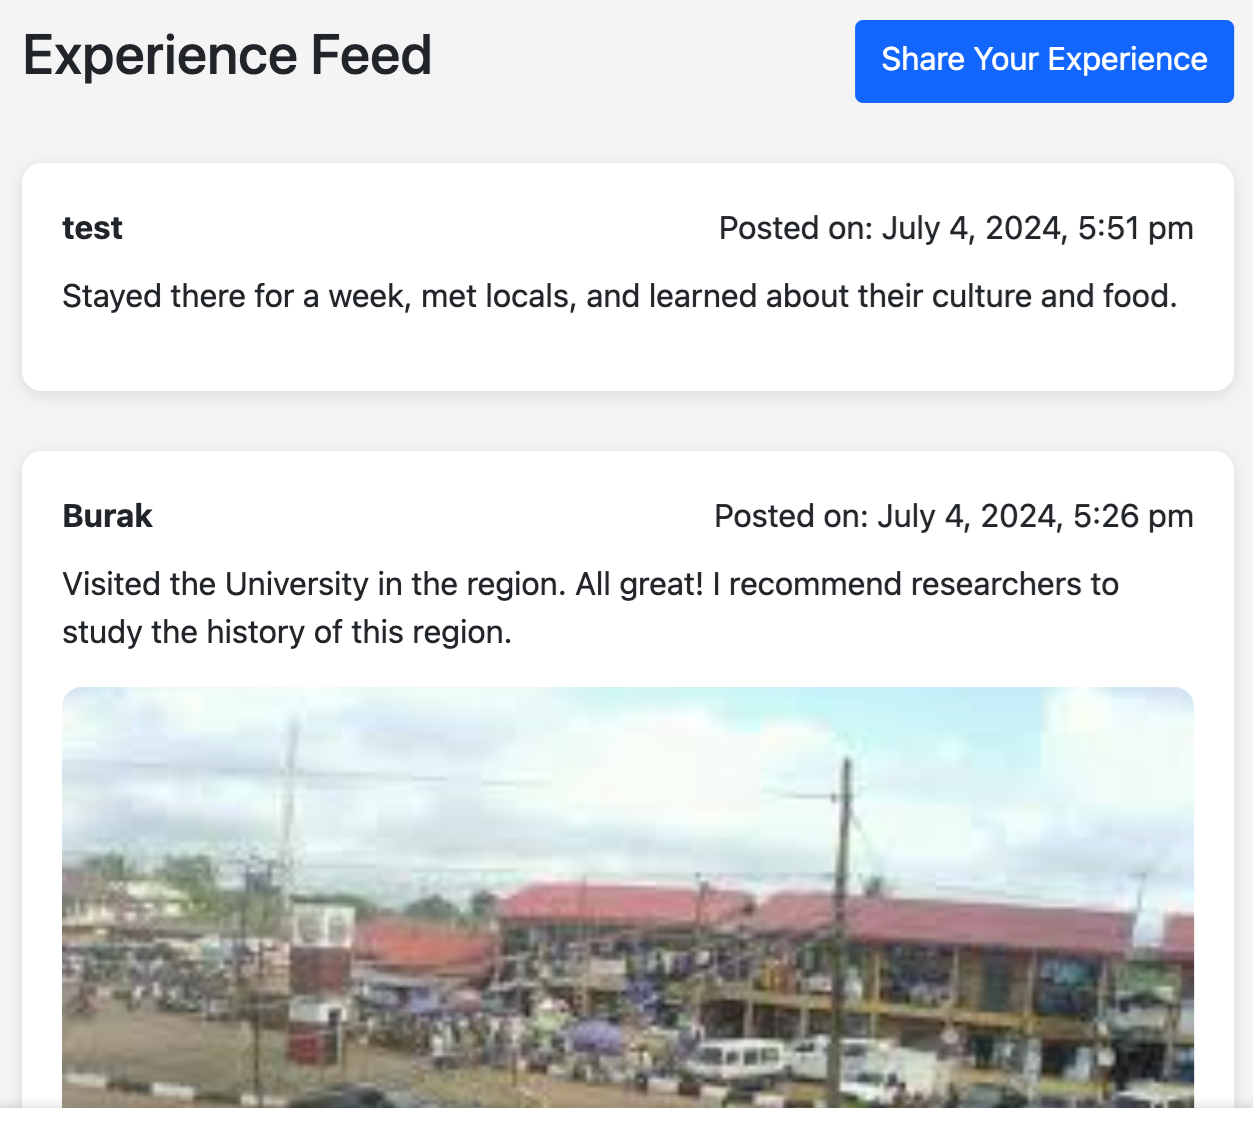
\includegraphics[width=\textwidth]{experienceFeed.png}
    \caption{Experience Feed}
    \label{fig:experienceFeed}
\end{figure}

\section{Share Your Experience}
This section allows users to post their personal experiences about places they have visited. They can share their stories, photos, and videos to help others learn more about these places.

\begin{figure}[H]
    \centering
    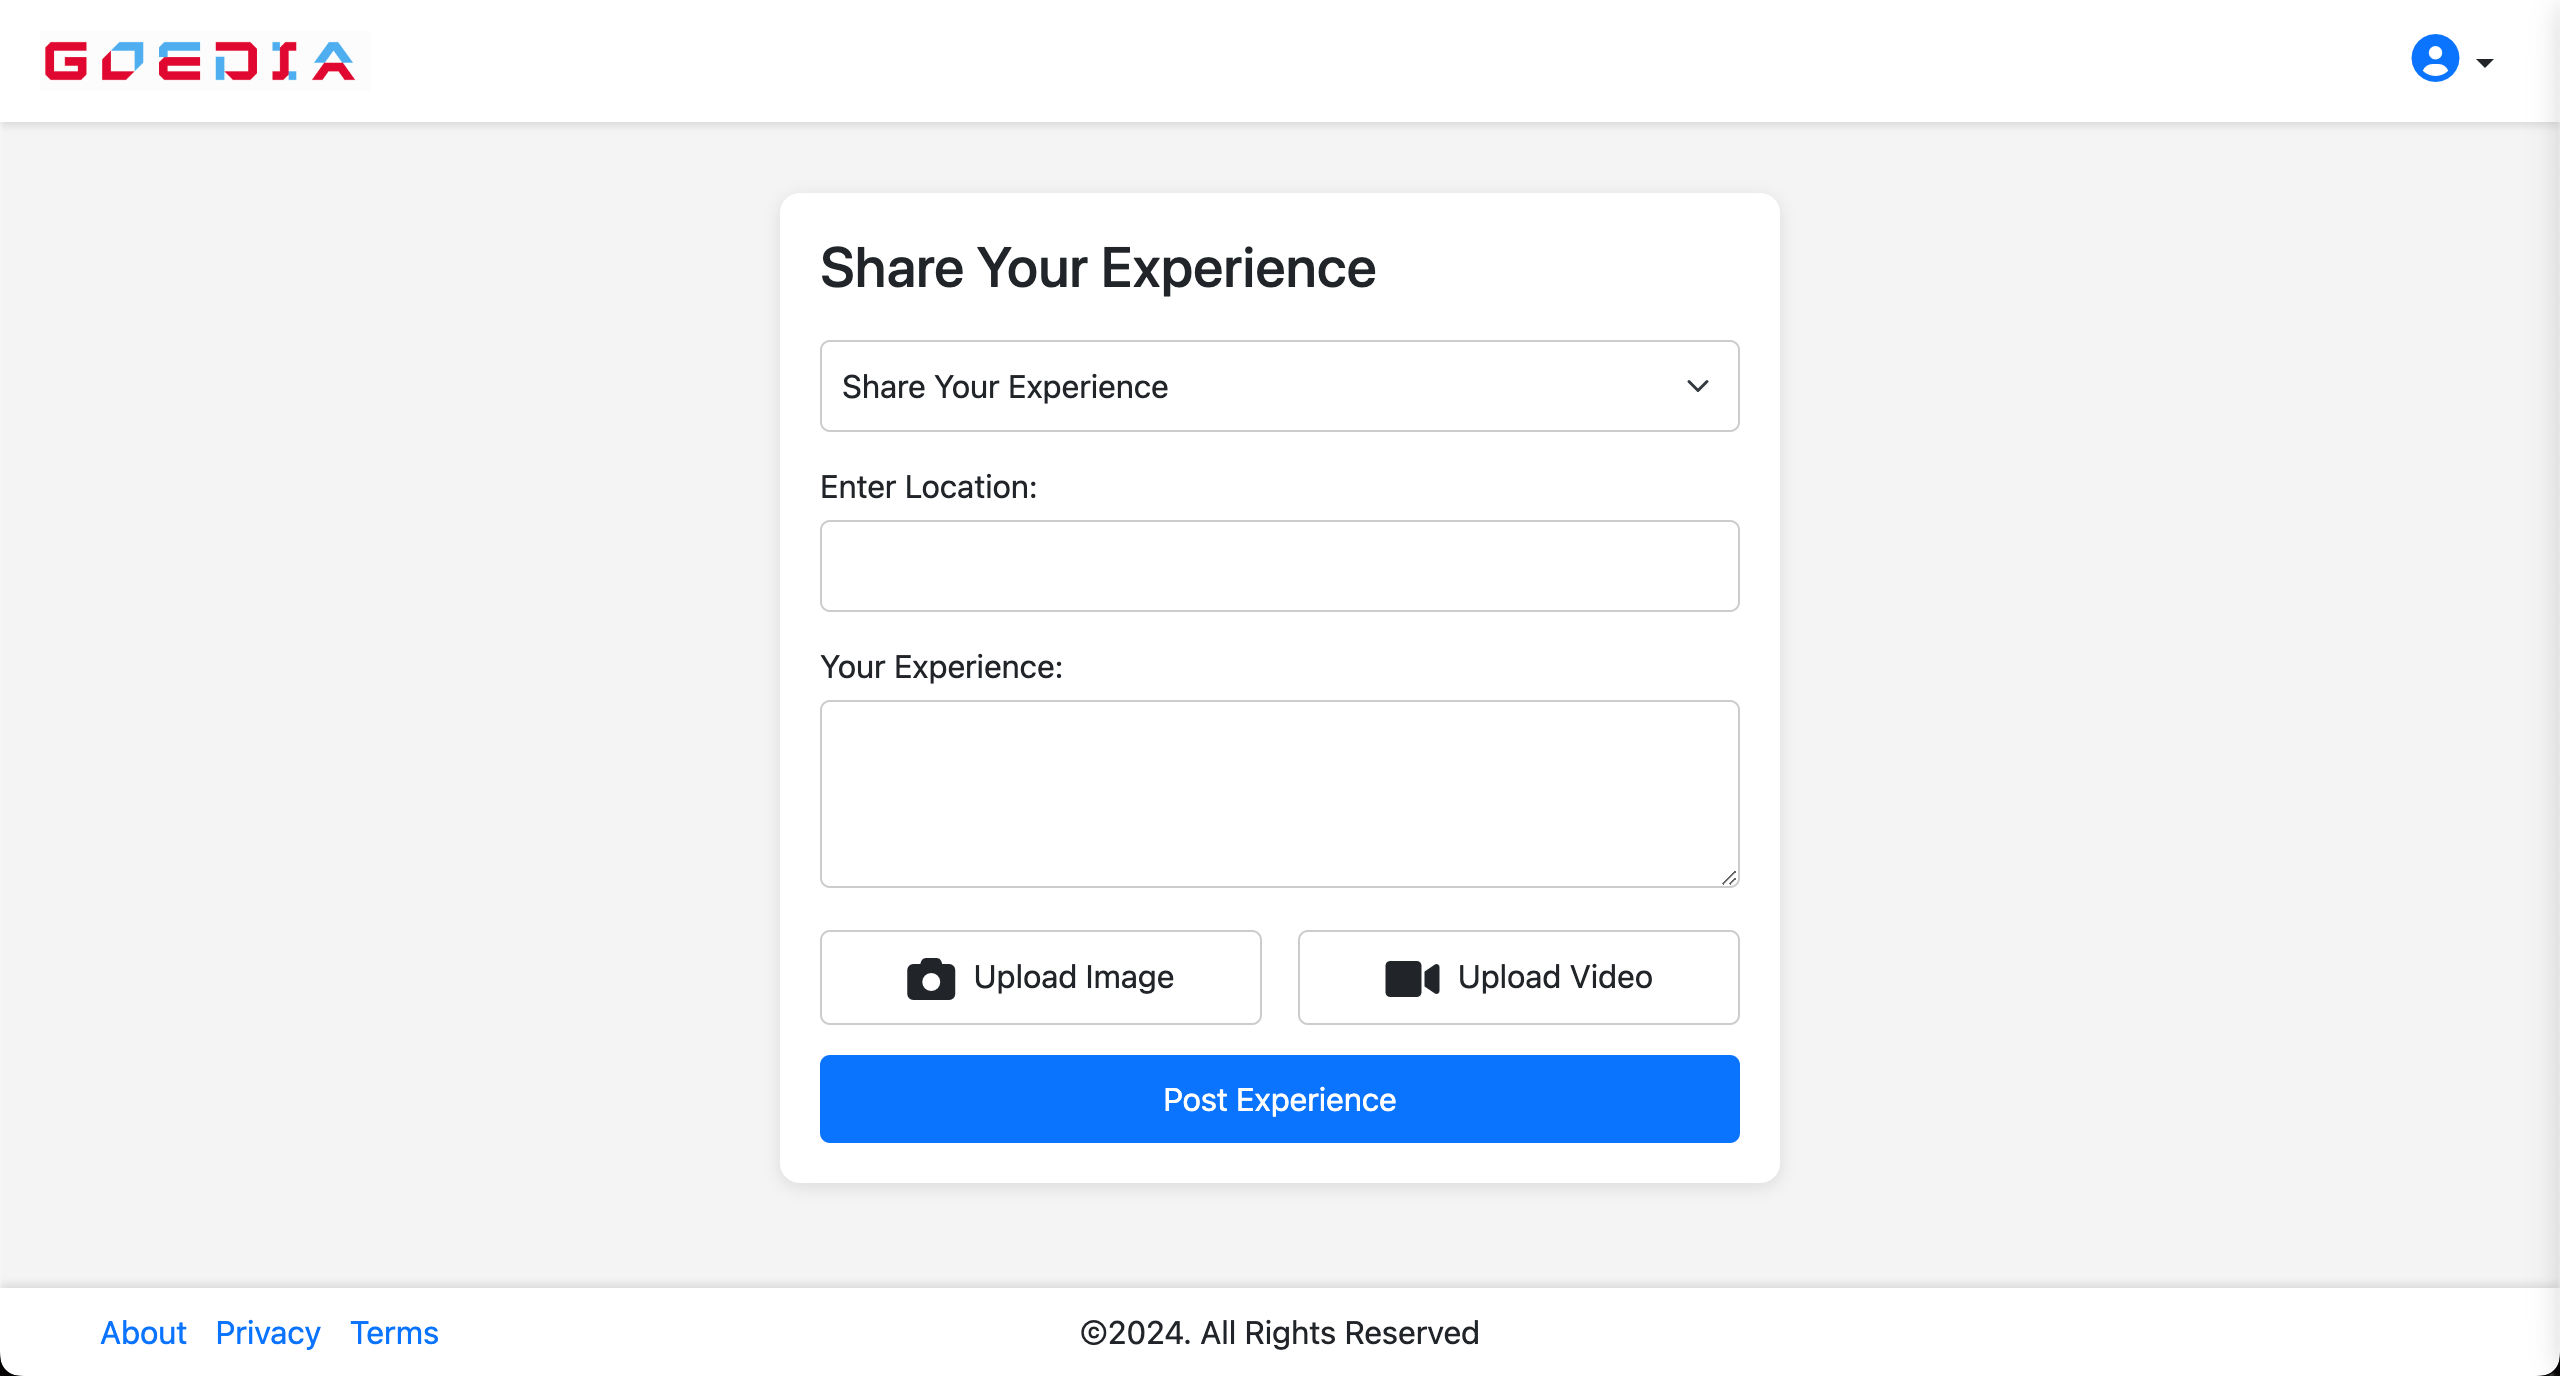
\includegraphics[width=\textwidth]{shareYourexperience.png}
    \caption{Share Your Experience}
    \label{fig:shareYourexperience}
\end{figure}

\section{Administrator Login}
Administrators have a separate login page to access additional functionalities for managing the application. This ensures secure access to administrative features.

\begin{figure}[H]
    \centering
    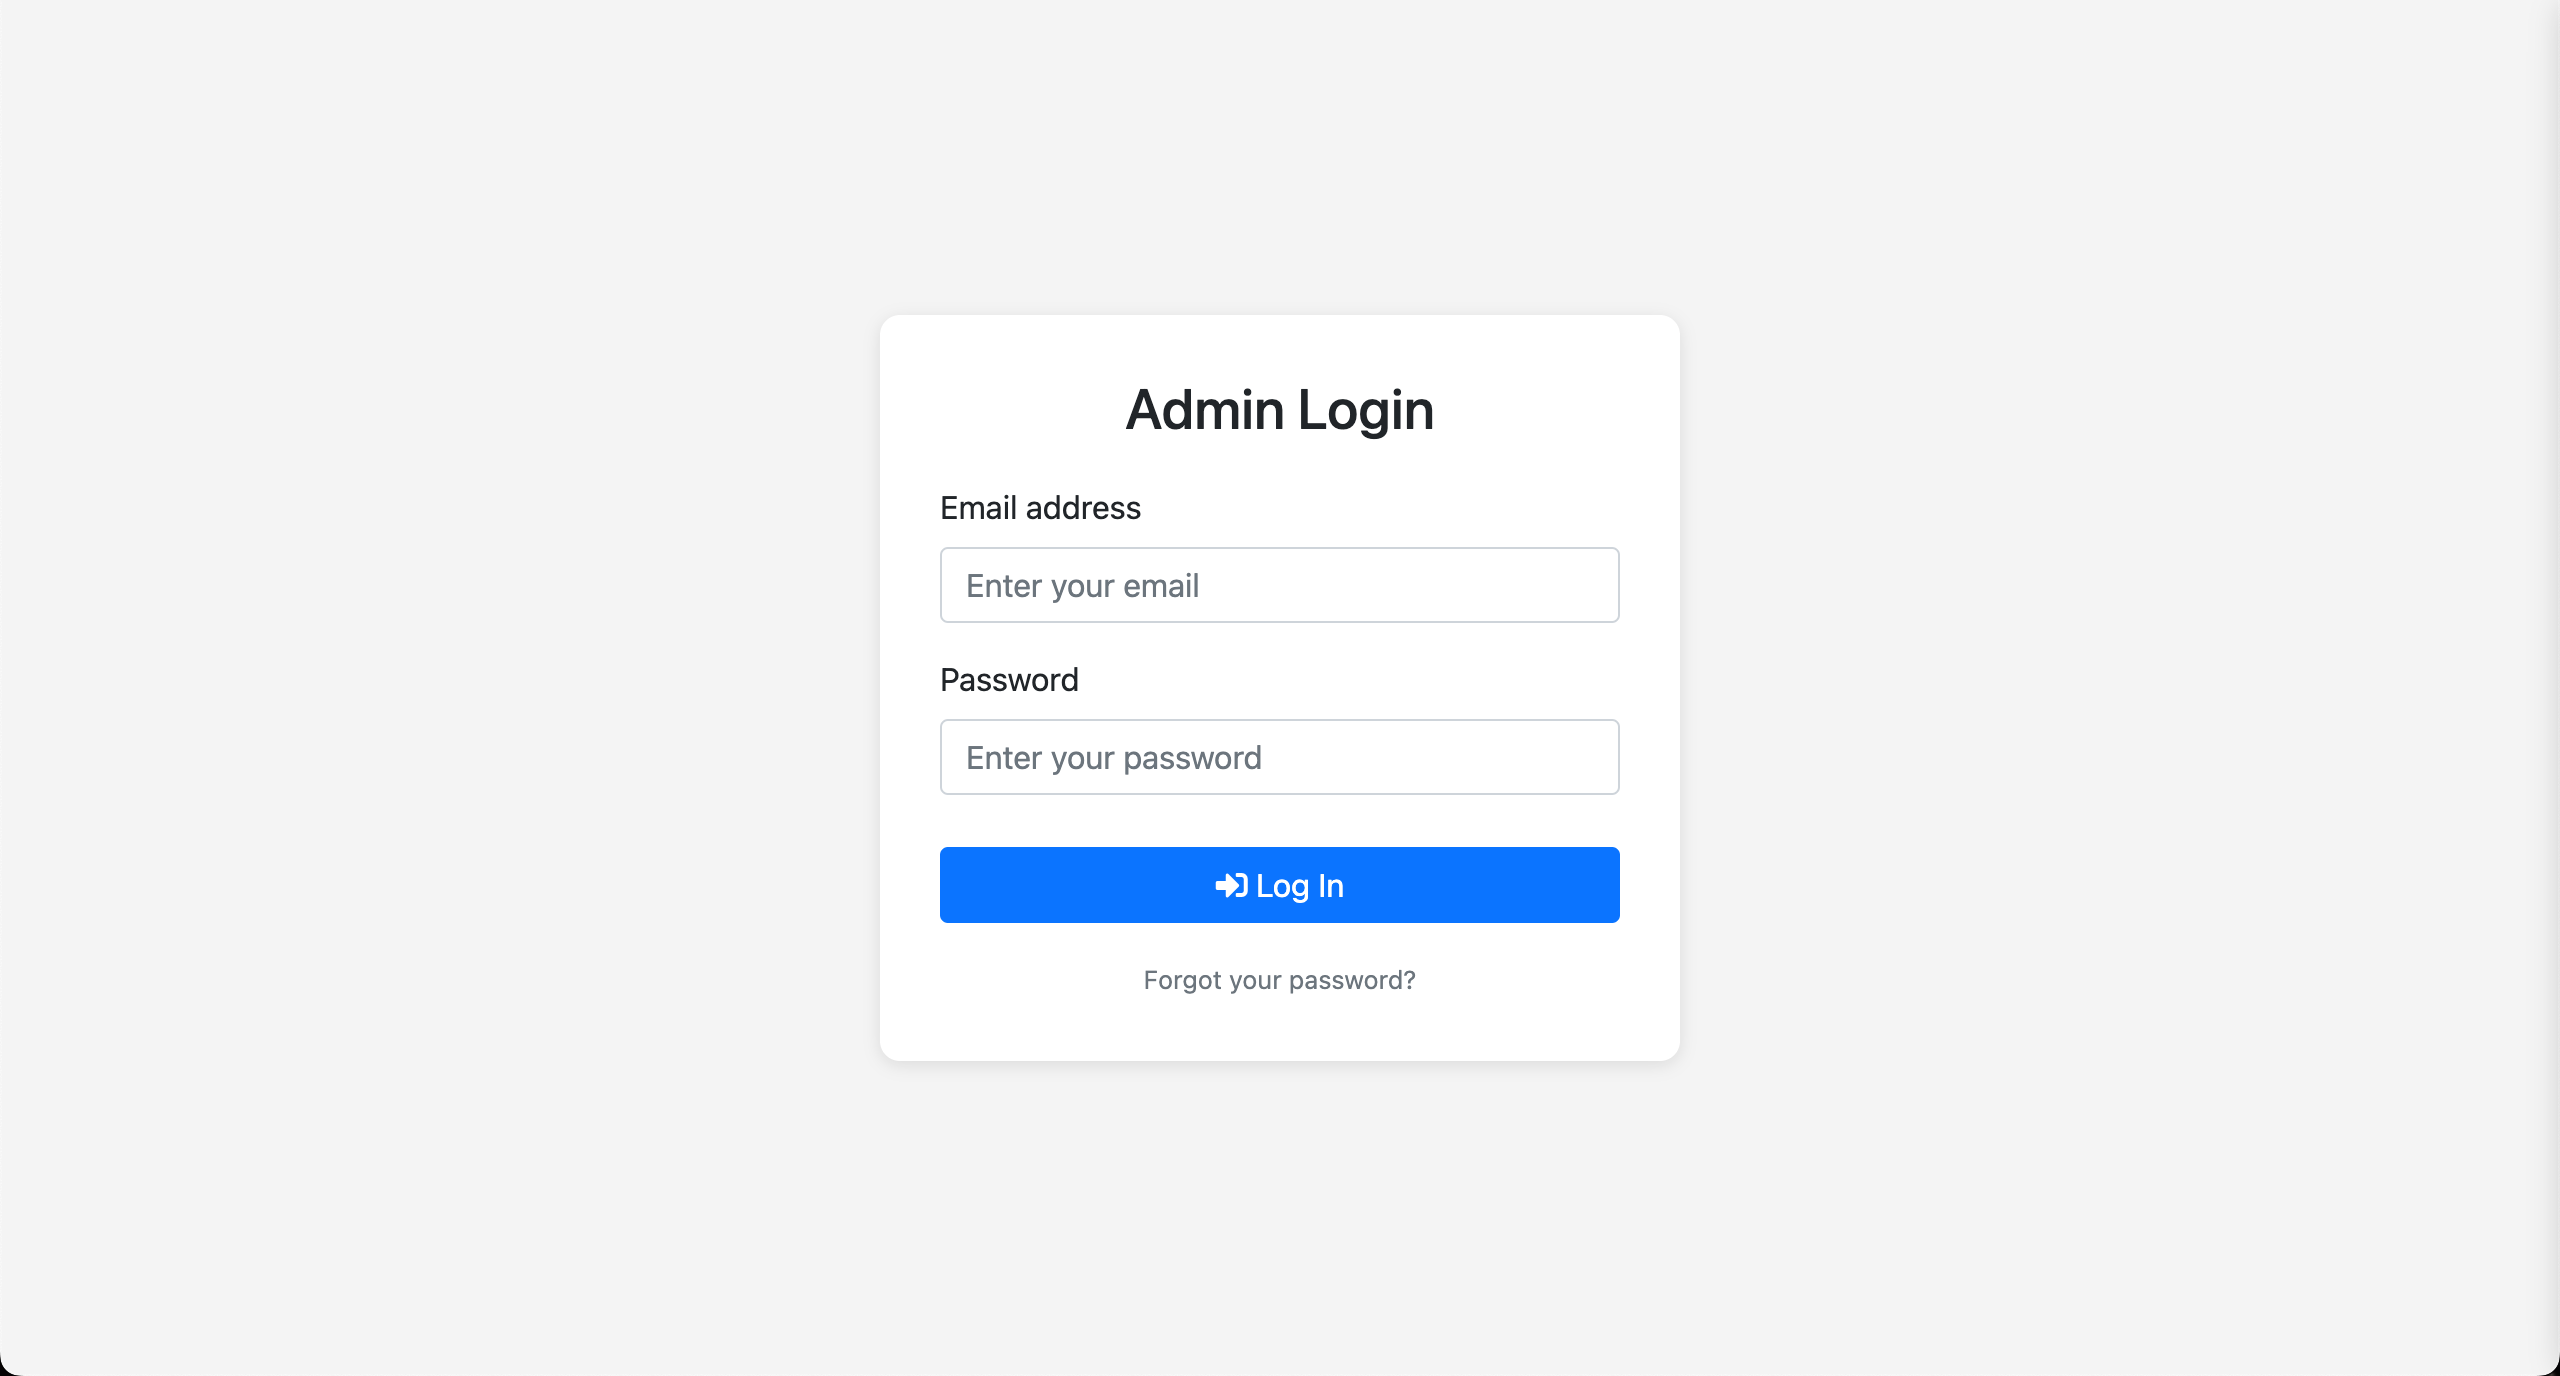
\includegraphics[width=\textwidth]{adminLogin.png}
    \caption{Administrator Login}
    \label{fig:adminLogin}
\end{figure}

\section{Administrator Dashboard}
The admin dashboard provides an overview of various metrics and functionalities that administrators can manage. This includes user management, content moderation, and site analytics.

\begin{figure}[H]
    \centering
    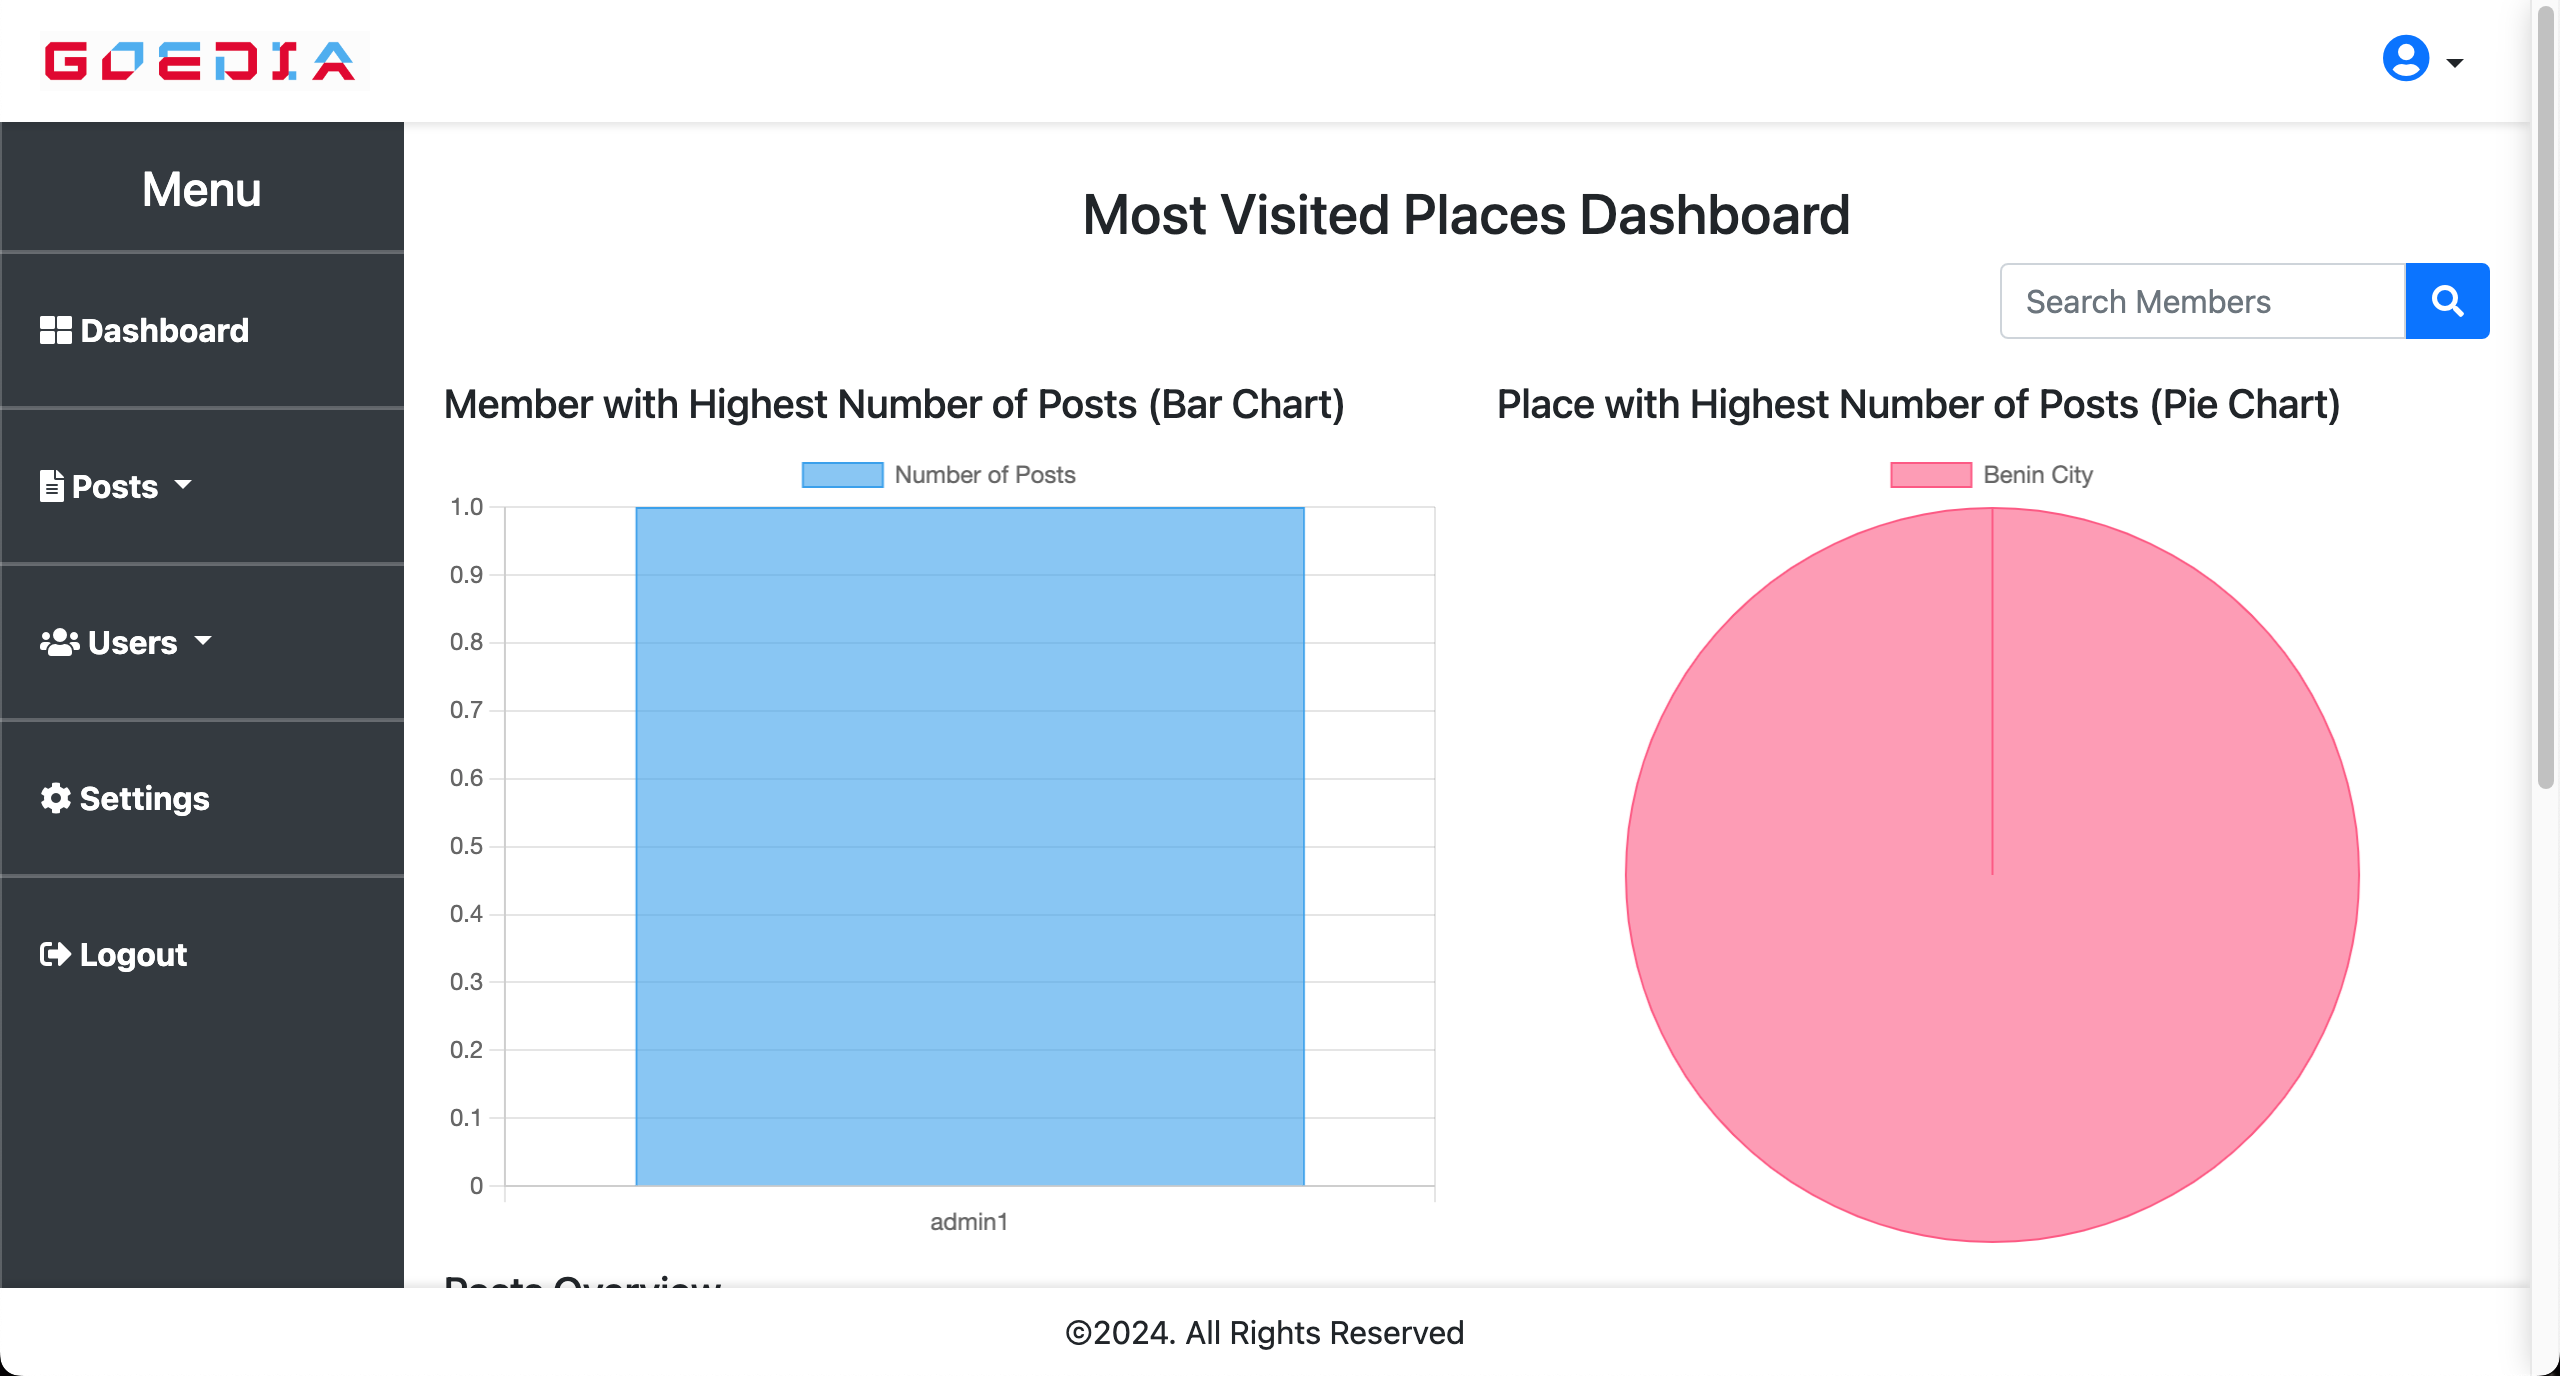
\includegraphics[width=\textwidth]{adminDash.png}
    \caption{Administrator Dashboard}
    \label{fig:adminDash}
\end{figure}

\section{Administrator Dashboard - Extended View}
A more detailed view of the admin dashboard with additional metrics and options. Administrators can perform advanced tasks and get a deeper insight into the site's performance.

\begin{figure}[H]
    \centering
    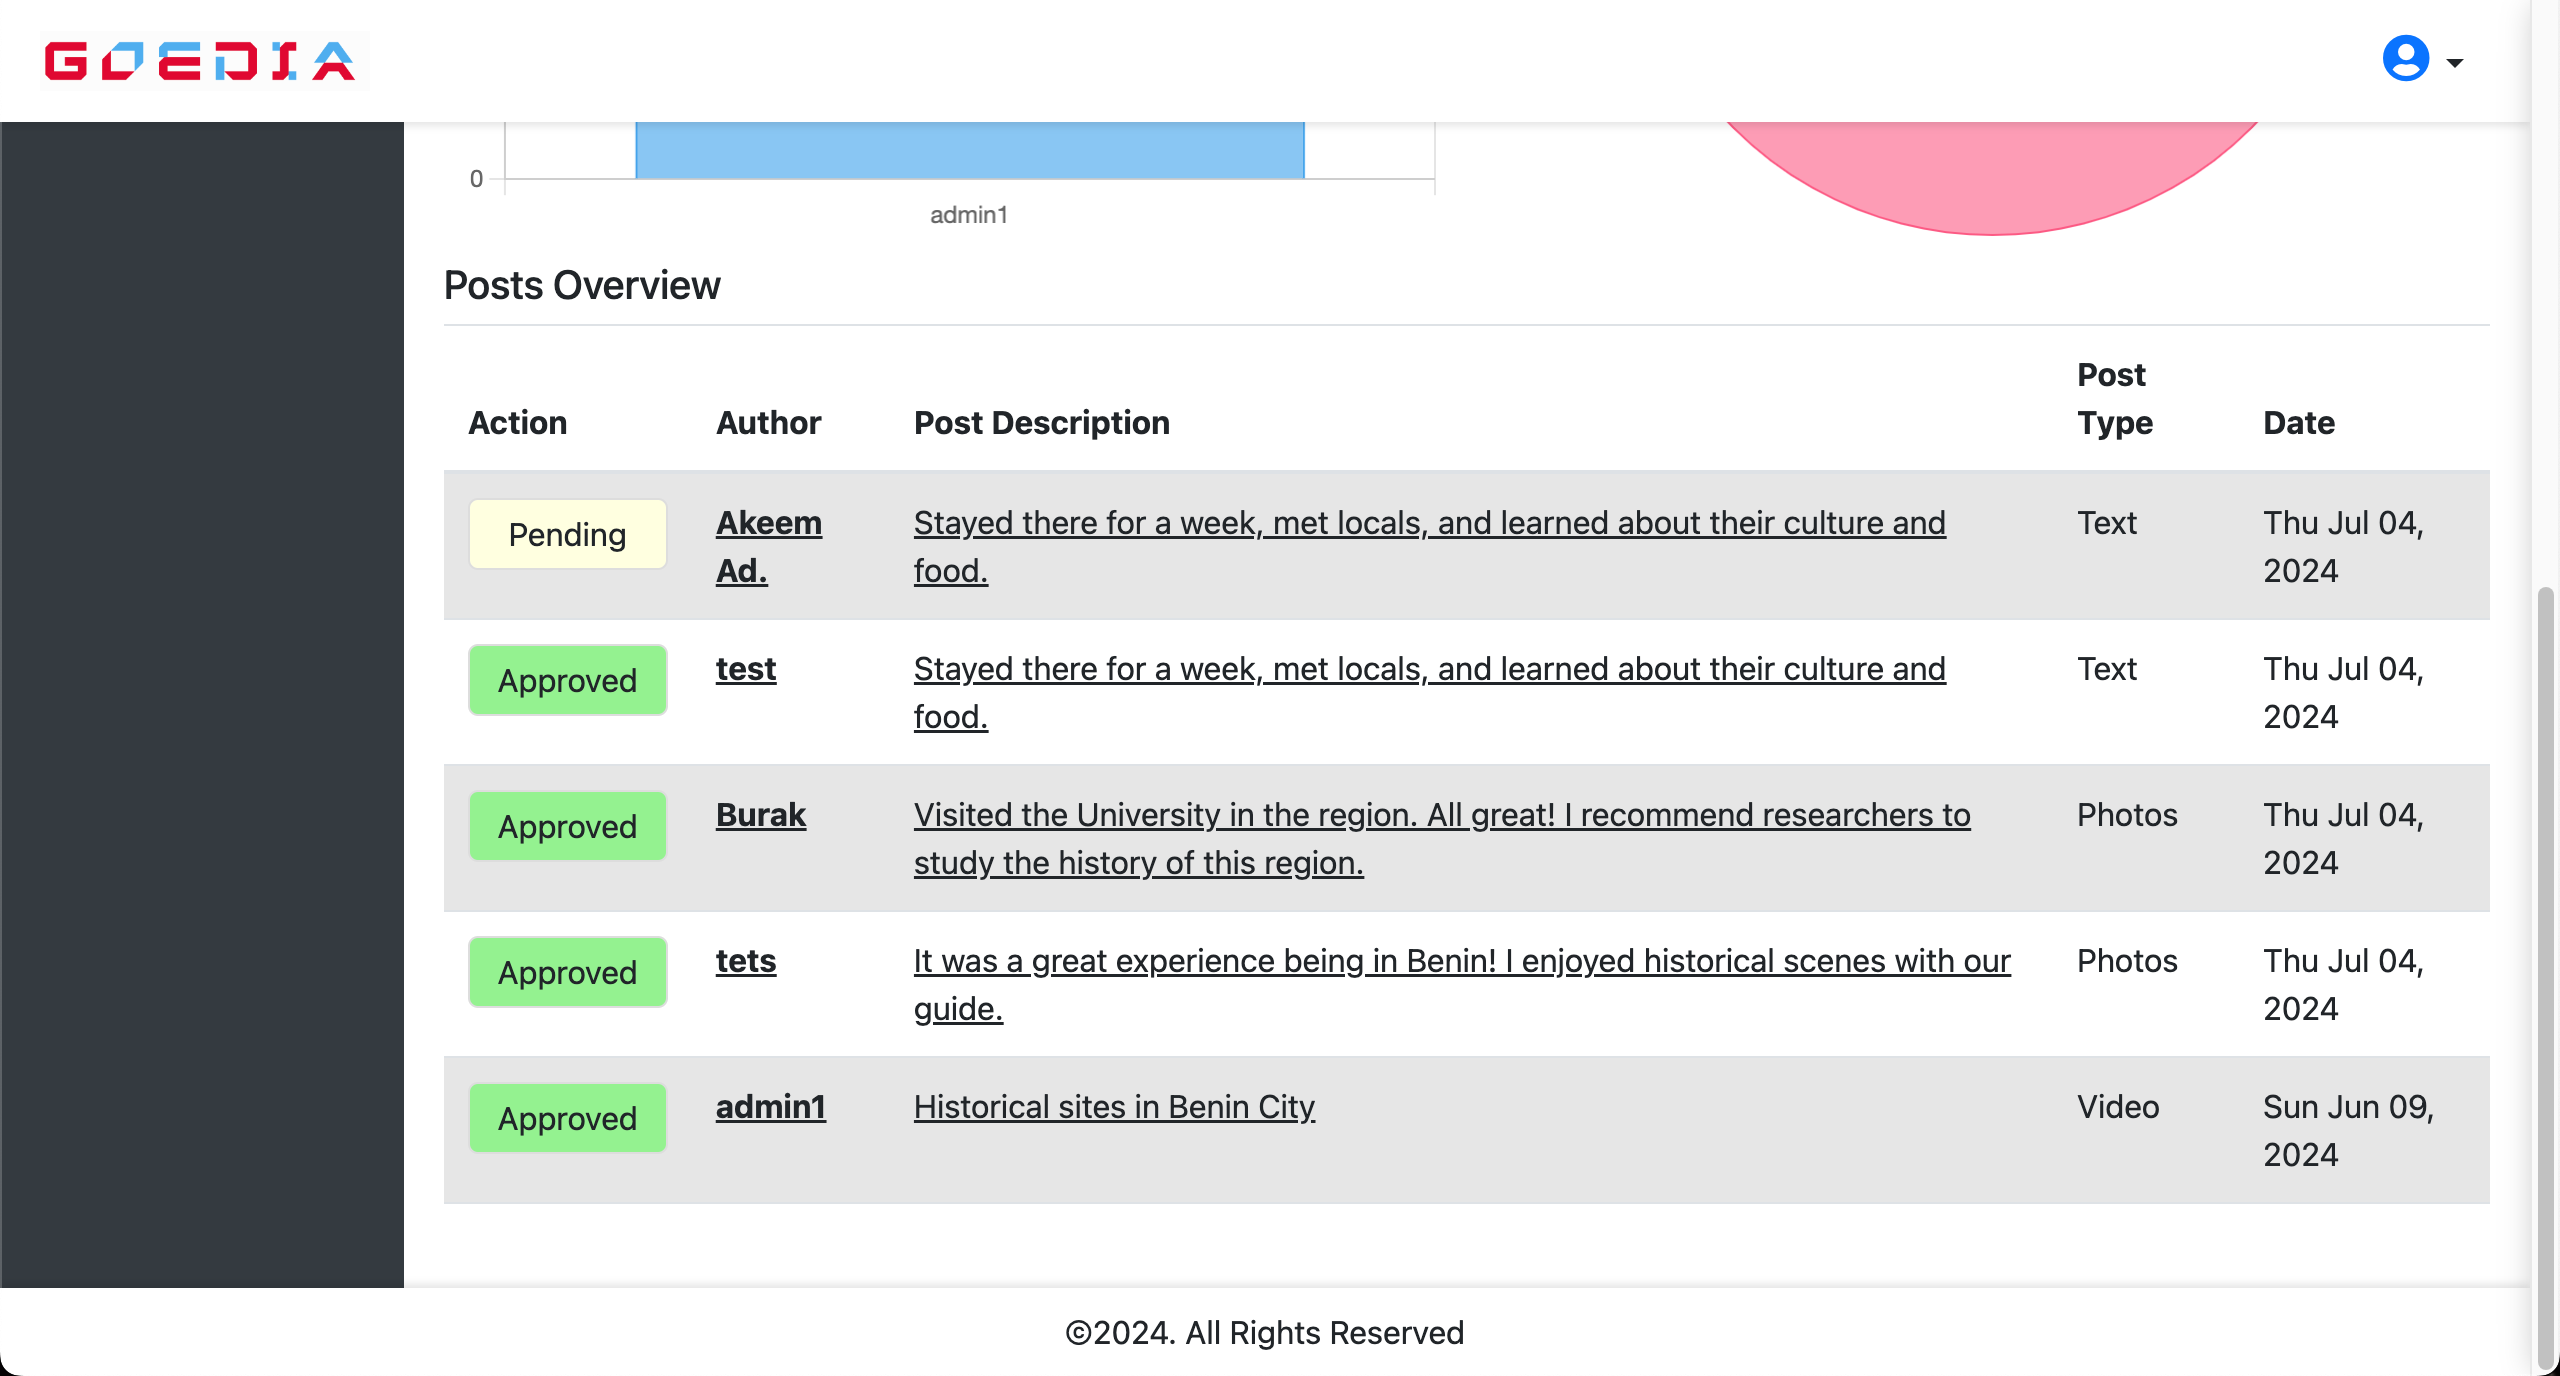
\includegraphics[width=\textwidth]{adminDash2.png}
    \caption{Administrator Dashboard - Extended View}
    \label{fig:adminDash2}
\end{figure}

\section{Admin Posts Management}
Administrators can manage user posts, including viewing, editing, and deleting posts if necessary. This ensures the content remains appropriate and useful for all users.

\begin{figure}[H]
    \centering
    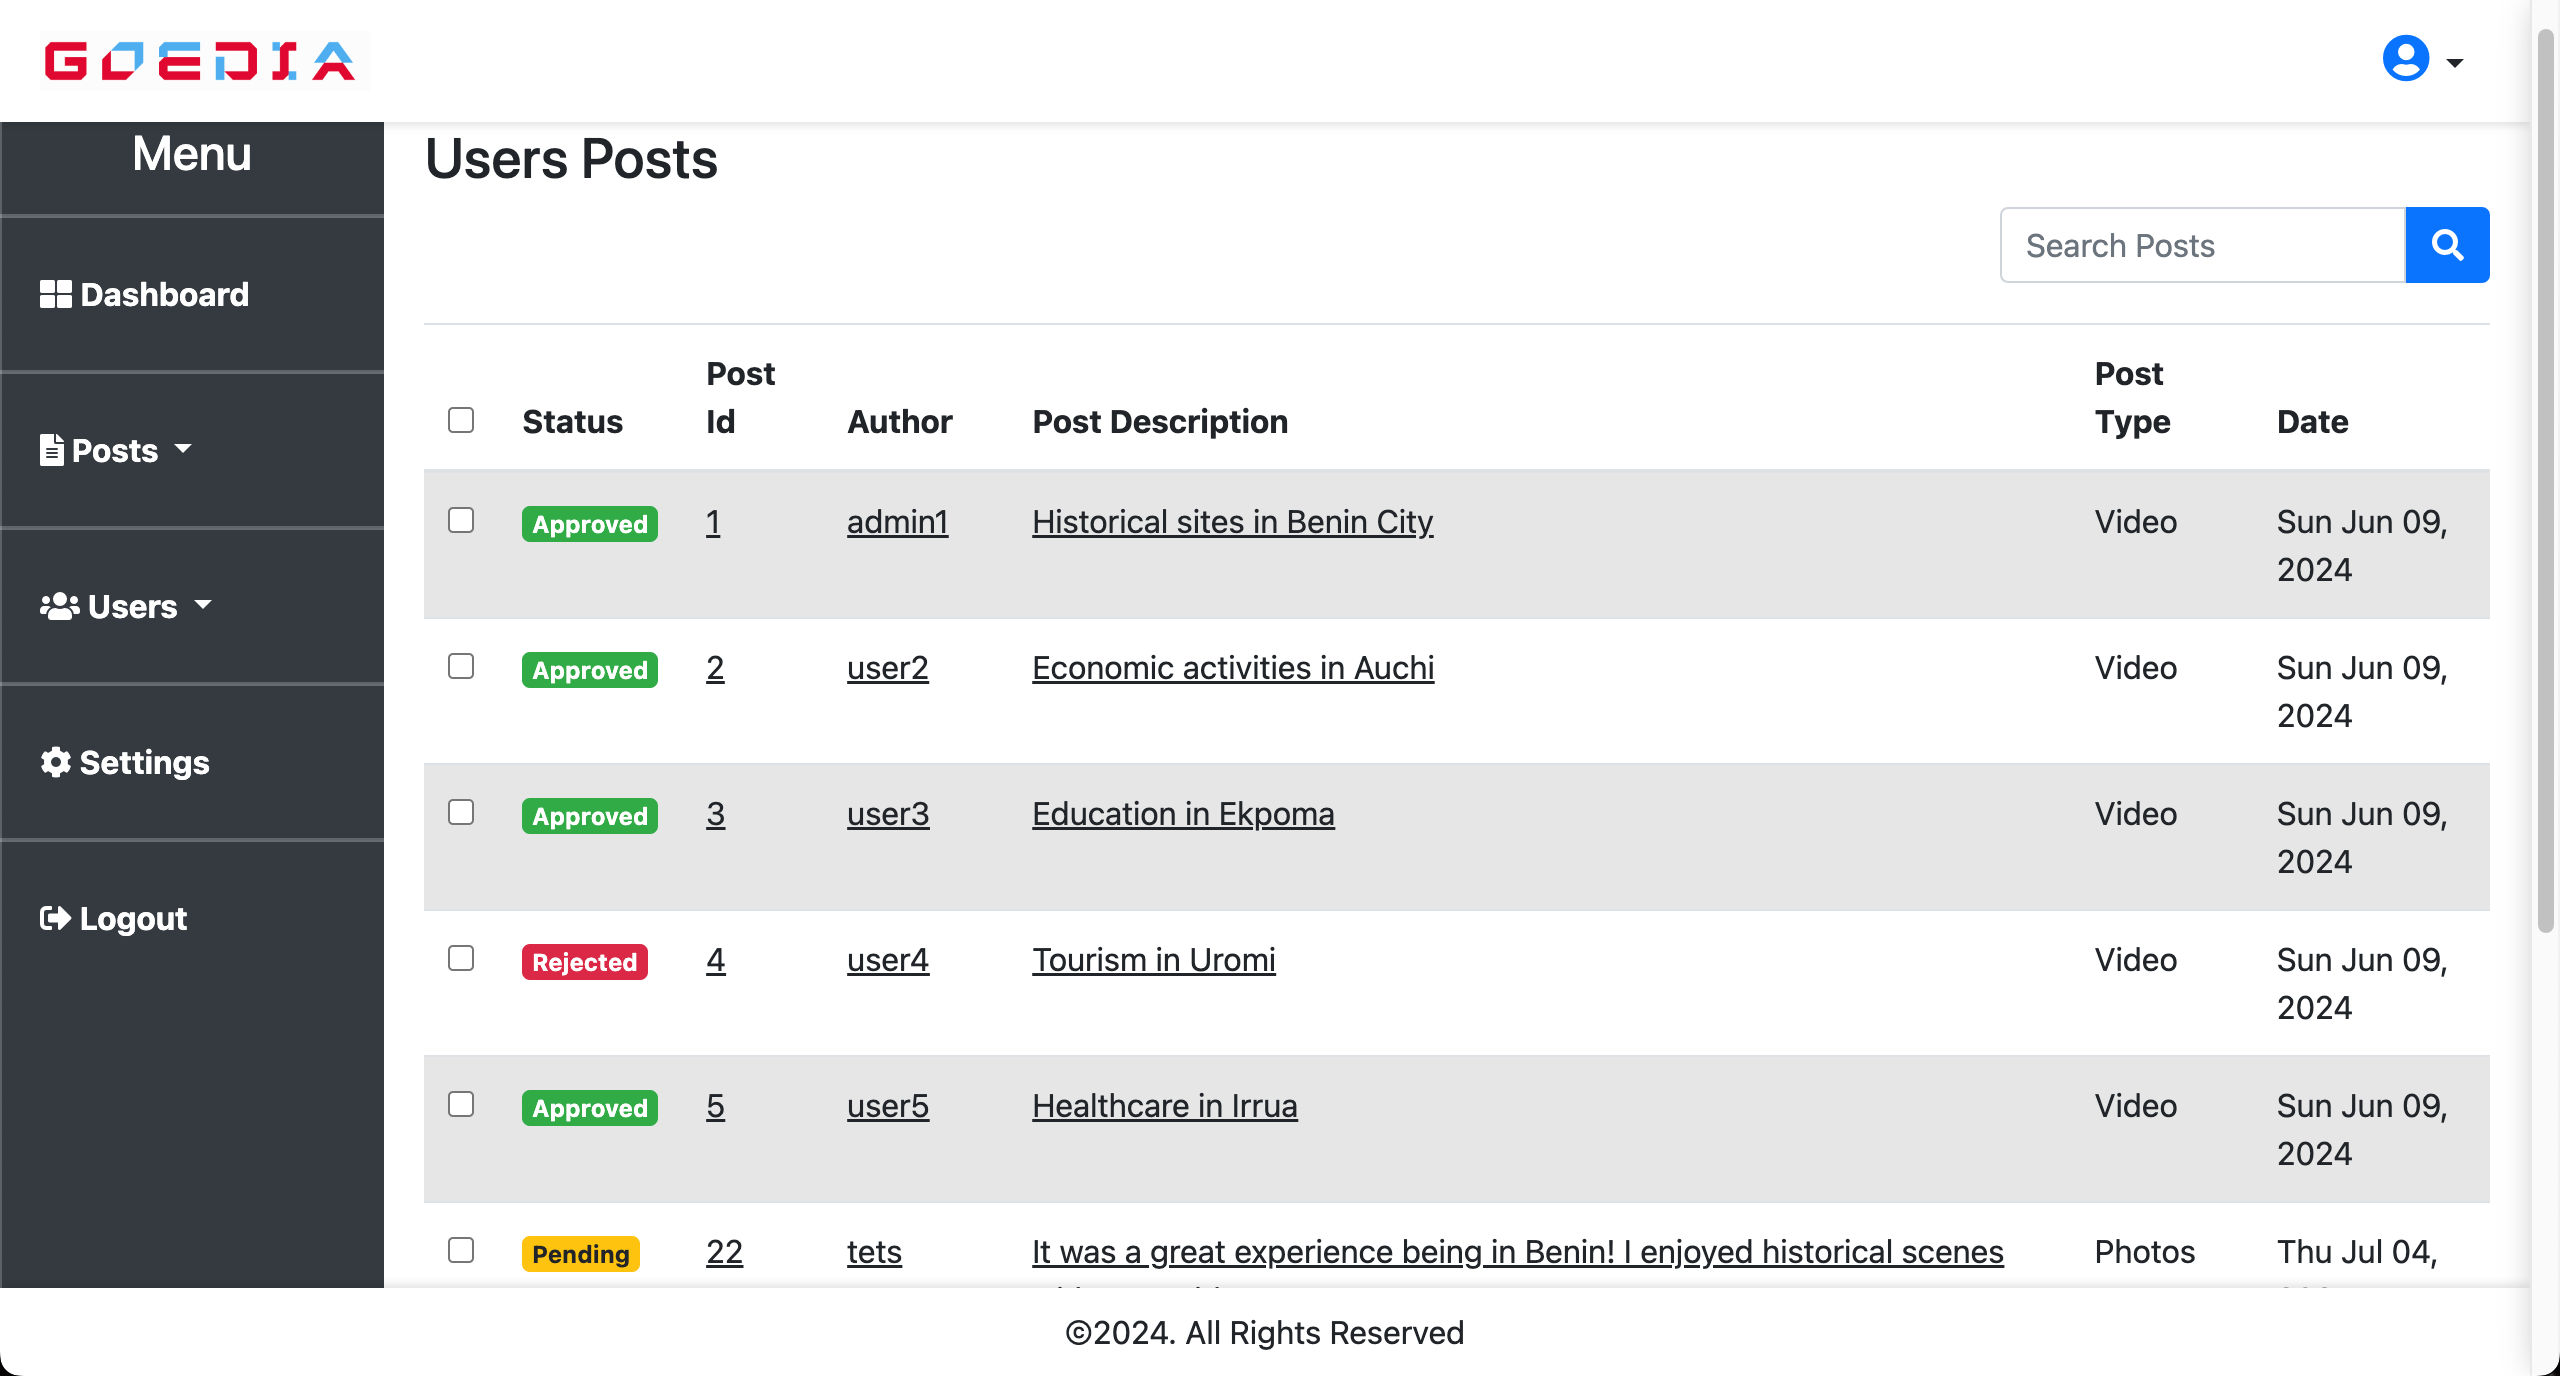
\includegraphics[width=\textwidth]{adminPOSTS.png}
    \caption{Admin Posts Management}
    \label{fig:adminPOSTS}
\end{figure}
